 \documentclass[journal]{IEEEtran}
\usepackage{authblk} % Required for adding multiple author affiliations
\IEEEoverridecommandlockouts

%%%%%%%%%%%%%%%%%%%%%%%%%%%%%%%%%%%%%%
%%%%%%%% PRINCIPALES PAQUETES %%%%%%%%
%      No modificar esta area        %
%%%%%%%%%%%%%%%%%%%%%%%%%%%%%%%%%%%%%%
\usepackage{fancyhdr}
\usepackage{graphicx}
%\usepackage[spanish, es-tabla]{babel}
\usepackage[english, spanish, es-tabla]{babel}
\usepackage[utf8]{inputenc}
\usepackage{color}
%\usepackage{hyperref}
\usepackage[hidelinks]{hyperref} 
\usepackage{wrapfig}
\usepackage{array}
\usepackage{multirow}
\usepackage{adjustbox}
\usepackage{nccmath}
\usepackage{subfigure}
\usepackage{amsfonts,latexsym} % para tener disponibilidad de diversos simbolos
\usepackage{enumerate}
\usepackage{booktabs}
\usepackage{float}
\usepackage{threeparttable}
\usepackage{array,colortbl}
\usepackage{ifpdf}
\usepackage{rotating}
%\usepackage{cite}
\usepackage{stfloats}
\usepackage{url}
\usepackage{listings}

\usepackage{capt-of}
%%%%%%%%%%%%%%%%%%%%%%%%%%%%%%%%%%%%%%%%%%%
%%%%%%%%%%%%%%%%%%%%%%%%%%%%%%%%%%%%%%%%%%%
%%% CREAR Y REESCRIBIR ALGUNOS COMANDOS %%%
%              No modificar esta area     %
%%%%%%%%%%%%%%%%%%%%%%%%%%%%%%%%%%%%%%%%%%%
\renewcommand\IEEEkeywordsname{Palabras clave}
%%%%%%%%%%%%%%%%%%%%%%%%%%%%%%%%%%%%%%%%%%%
%%%%%%%%%%%%%%%%%%%%%%%%%%%%%%%%%%%%%%%%%%%
%%%           CONFIGURACION             %%%
%              No modificar esta area     %
%%%%%%%%%%%%%%%%%%%%%%%%%%%%%%%%%%%%%%%%%%%
% correct bad hyphenation here
\hyphenation{op-tical net-works semi-conduc-tor} %% Con este comando se especifican como pueden seprarse las sílabas adecuadamente en caso una palabra quede en dos lineas diferentes de texto
\graphicspath{ {figs/} }  %%Ruta donde se encuentran las imágenes, que esté vacio indica que las imagenes están dentro de la misma carpeta que contiene el archivo .tex

%%%%%%%%%%%%%%%%%%%%%%%%%%%%%%%%%%%%%%%%%%
%%%   TITULO Y LOGOS DE PRIMERA PAGINA %%%
%%%%%%%%%%%%%%%%%%%%%%%%%%%%%%%%%%%%%%%%%%

% ---- Archivos de los escudos ----
\newcommand{\LogoIzq}{figs/escudos/escudo-ciencias.png}
\newcommand{\LogoDer}{figs/escudos/escudo-if.png}

% ---- Altura de los escudos ----
% Se pueden ajustar independientemente debido a que las imágenes
% pueden tener diferentes proporciones o márgenes internos.
\newcommand{\AlturaLogoIzq}{3cm}
\newcommand{\AlturaLogoDer}{3.2cm}


% ---- Construcción del título de la primera página ----
%
% Distribución horizontal:
%
% | 18 % logo UNAM | 64 % título | 18 % logo Ciencias |
%
% De esta forma los logos permanecen junto a los márgenes mientras
% que el título dispone siempre de una zona independiente.
%
\newcommand{\firstpagetitle}[1]{%
	\makebox[\textwidth][c]{%
		%
		% Logo izquierdo
		\parbox[c]{0.18\textwidth}{%
			\raggedright
			\includegraphics[
			width=0.95\linewidth,
			height=\AlturaLogoIzq,
			keepaspectratio
			]{\LogoIzq}%
		}%
		%
		% Título
		\parbox[c]{0.64\textwidth}{%
			\centering
			\textcolor{black}{#1}\par
		}%
		%
		% Logo derecho
		\parbox[c]{0.18\textwidth}{%
			\raggedleft
			\includegraphics[
			width=0.95\linewidth,
			height=\AlturaLogoDer,
			keepaspectratio
			]{\LogoDer}%
		}%
	}%
}


% ---- Modificar \title ----
%
% En main.tex solamente será necesario escribir:
%
% \title{Nombre de la práctica}
%
\let\OriginalReportTitle\title

\renewcommand{\title}[1]{%
	\OriginalReportTitle{%
		\firstpagetitle{#1}%
	}%
}


% ---- Evitar que Hyperref intente meter los logos en los metadatos PDF ----
\pdfstringdefDisableCommands{%
	\def\firstpagetitle#1{#1}%
}


% ---- Estilo de la primera página ----
% Se mantiene para que no aparezcan encabezados ni pies de página,
% pero los logos YA NO pertenecen a fancyhdr.
\fancypagestyle{firstpage}{%
	\fancyhf{}%
	\renewcommand{\headrulewidth}{0pt}%
}

\begin{document}

%%%%%% Titulo %%%%%
\title{\textcolor{black}{Propiedades ópticas en tierras raras}}  

%%%%% Datos %%%%%
\author{Juan Alexis Hernández Hernández}
\author{Ashley Stacy Rosas Galicia\\
\texttt{Correos: alexi5@ciencias.unam.mx y ashphyrosas@ciencias.unam.mx}}
\affil{Facultad de Ciencias, Universidad Nacional Autónoma de México, Circuito Exterior s/n, Ciudad Universitaria, Ciudad de México. C. P. 04510 \\ \vspace*{14pt} \fontsize{11}{6}\selectfont 11 de octubre de 2026}

\twocolumn[
\begin{@twocolumnfalse}
\maketitle
\thispagestyle{firstpage}
\end{@twocolumnfalse}

%%%%% Resumen ESPAÑOL%%%%%
\begin{abstract}
Se estudió la fotoluminiscencia de materiales dopados con iones de tierras
raras mediante el análisis de sus espectros de emisión. Las muestras se midieron con dos configuraciones
experimentales: un espectrómetro PerkinElmer LS55 y un espectrómetro
Ocean Optics acoplado a una fibra óptica. Para cada banda identificada
se estimó la longitud de onda máxima y su incertidumbre a partir de la
anchura a media altura; posteriormente, se calcularon los números de onda
y sus incertidumbres por propagación. En el vidrio de fosfato de zinc
dopado con Sm$^{3+}$ se observaron máximos en
$566.0 \pm 13.5$, $602.5 \pm 14$,
$648 \pm 14$ y $708\pm 20\,\text{nm}$.
Con el segundo aparato se obtuvieron bandas en
$562.2\pm 9.5$, $598.6\pm 0.3$, $645\pm 0.3$ y $705.4\pm 41.2\ ,\text{nm}$
La cercanía entre ambos conjuntos concuerda con que se midió el mismo
material, aunque las diferencias pueden relacionarse con la resolución
y calibración de los equipos. También se observaron variaciones en las
bandas de emisión del Dy$^{3+}$ al incorporarlo en distintas matrices.
En el vidrio de tetraborato de litio dopado con Tb$^{3+}$ se encontraron máximos en $492 \pm 18$, $547.5 \pm 11.5$,
$590 \pm 16.5$ y $625.5 \pm 12.5\,\text{nm}$, mientras que en el cristal de metafostato y ortofosfato de magnesio co-dopado con cloruro de sodio y Eu$^{3+}$ se obtuvieron máximos en $611.52 \pm 5.21$, $592.02 \pm 13.28$,
$701.71 \pm 7.40$ y $653.22\pm 24.62\,\text{nm}$ y en el cristal de praseodimio se encontraron máximos en $609.44 \pm 33.96$, $640.88 \pm 8.59$,
$490.49 \pm 18.02$, $525.64\pm 30.25\,$ y $723.12 \pm 1 \text{nm}$.
En conjunto, los resultados muestran que la matriz anfitriona y las
condiciones instrumentales deben considerarse al interpretar los
espectros. Las incertidumbres reportadas son estimaciones visuales de
la anchura de las bandas y no representan la incertidumbre instrumental.
\vspace{2mm}

%%%%% Palabras clave ESPAÑOL%%%%%
\begin{IEEEkeywords}
tierras raras; fotoluminiscencia;
espectros de emisión; transiciones ópticas; samario; disprosio.
\end{IEEEkeywords}
\end{abstract}
\bigskip

%%%%% Resumen INGLÉS%%%%%
\begin{otherlanguage}{english}
\begin{abstract}
The photoluminescence of rare-earth-doped materials was studied by
analyzing their emission spectra. The samples were measured using two
experimental configurations: a PerkinElmer LS55 spectrometer and an
Ocean Optics spectrometer coupled to an optical fiber. For each
identified emission band, the wavelength of the maximum and its
uncertainty were estimated from the full width at half maximum (FWHM);
the corresponding wavenumbers and their uncertainties were subsequently
calculated by error propagation. For the Sm$^{3+}$-doped zinc phosphate
glass, emission maxima were observed at $566.0 \pm 13.5$,
$602.5 \pm 14$, $648 \pm 14$, and $708 \pm 20\,\text{nm}$.
Measurements with the second instrument yielded bands at
$562.2 \pm 9.5$, $598.6 \pm 0.3$, $645 \pm 0.3$, and
$705.4 \pm 41.2\,\text{nm}$. The similarity between both sets of
wavelengths is consistent with measurements of the same material,
although the differences may be related to the resolution and
calibration of the instruments. Variations in the Dy$^{3+}$ emission
bands were also observed when the ion was incorporated into different
host matrices. For the Tb$^{3+}$-doped lithium tetraborate glass,
emission maxima were found at $492 \pm 18$, $547.5 \pm 11.5$,
$590 \pm 16.5$, and $625.5 \pm 12.5\,\text{nm}$. In the magnesium
metaphosphate and orthophosphate crystal co-doped with sodium chloride
and Eu$^{3+}$, emission maxima were obtained at
$611.52 \pm 5.21$, $592.02 \pm 13.28$, $701.71 \pm 7.40$, and
$653.22 \pm 24.62\,\text{nm}$. For the praseodymium crystal,
emission maxima were found at $609.44 \pm 33.96$,
$640.88 \pm 8.59$, $490.49 \pm 18.02$, $525.64 \pm 30.25$, and
$723.12 \pm 1\,\text{nm}$. Overall, the results show that both the
host matrix and the instrumental conditions should be considered when
interpreting the emission spectra. The reported uncertainties are
visual estimates of the band widths and do not represent instrumental
uncertainty.
	\vspace{2mm}
	
%%%%% Palabras clave INGLÉS%%%%%
\renewcommand\IEEEkeywordsname{Keywords}
\begin{IEEEkeywords}
	rare earths; photoluminescence; emission
spectra; optical transitions; samarium; dysprosium.
\end{IEEEkeywords}
\end{abstract}
\end{otherlanguage}
\bigskip
]

%%%%% Partes del reporte %%%%%
\textcolor{black}{\section{Introducción}}

\noindent Las tierras raras están conformadas por 17 elementos de la tabla periódica. En el último tercio del siglo presente, se ha logrado obtener cantidades suficientes de tierras raras con elevada pureza que ha dado lugar a materiales avanzados o tecnologías presentes hoy en la vida cotidiana. Algunos ejemplos son, materiales ópticos (tales como las fibras, los pogmentos, etc.), pantallas de televisión, imanes permanentes y catalizadores\cite{Cheng2018}. 
Las propiedades que hacen que las tierras raras sean de interés están íntimamente relacionadas con su configuración electrónica. Sus electones de interés óptico se encuentran principalmente en la subcapa \textit{4f}, la configuración electrónica general del átomo neutro es de la forma: \([Xe]\,4f^n6s^2\). Cuando se habla de tierras raras, normalmente nos interesa hablar de la configuración electrónica del ión dopante, como omo \(Eu^{3+}\), \(Dy^{3+}\), \(Tb^{3+}\) o \(Nd^{3+}\). 
Ahora bien, los electrones \textit{4f} son responsables de algunas de las líneas de emisión que producen las tierras raras y los electrones de dichas capa están protegidos por capas más externas \textit{5s} y \textit{5p}\cite{Cheng2018}. Si los electrones \textit{4f} estuvieran totalmente expuestos al entorno en donde se introducen los iones dopantes, el campo eléctrico del entorno podría modificar las energías que se observan. Debido a esta protección, los niveles de energía de los niveles \textit{4f} suelen conservar características similares al ser introducidos a materiales distintos.
\subsection{Espectro de emisión}
Al incidir luz sobre un ión de tierra rara, el ión alcanza un estado de mayor energía y después regresa a un estado de menor energía, en este proceso puede ocurrir dos posibilidades; por relajación radiactiva, el electrón pasa a un estado de menor energía y emite un fotón con una energía igual a la diferencia de energía entre niveles, pot relajación no radiativa, el ion pierde energía que se transmite en forma de vibraciones al material o a otro ion. En la relajación no radiativa destacan la relajación multifonónica, la relajación cruzada y la conversión ascendente cooperativa\cite{RighiniFerrari2005}. Estos mecanismos pueden competir con la emisión luminosa y modificar tanto la intensidad de fluorescencia como la eficiencia cuántica del material.
En un espectro de emisión se registran las longitudes emitidas después de la exitación cuando se la relación radiativa, la asignación de las bandas a transiciones electrónica permite reconocer la respuesta característica de cada ion.
\subsection{Fluorescencia}
La fluorescencia es la emisión de luz de un material, que ocurre cuando un material absorbe energía y libera parte de en forma de luz. Se distingue de la fosforescencia por la rapidez en que ocurre la emisión una vez retirada la excitación. \cite{RighiniFerrari2005}
\subsection{Obejtivos}
En este trabajo se caracterizan las propiedades de emisión de los iones
Dy$^{3+}$ y Sm$^{3+}$ mediante el análisis de sus espectros de
fotoluminiscencia. Se identifican las principales bandas de emisión,
se determinan sus longitudes de onda y números de onda, y se relacionan
con las transiciones electrónicas correspondientes. Además, se compara
la emisión del Dy$^{3+}$ en dos matrices vítreas distintas para evaluar
la influencia del material anfitrión, y se contrastan las mediciones
del Sm$^{3+}$ obtenidas con dos aparatos diferentes para examinar la
consistencia de las posiciones de las bandas registradas.\\
\textcolor{black}{\section{Procedimiento}}

\begin{figure}%[H]
	\centering
	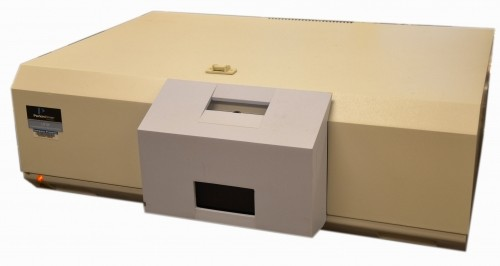
\includegraphics[scale=0.4]{figs/PELS55.jpg}
	\caption{Perkin Elmer LS55 Luminsescence Spectrometer. \cite{PELS55}}
	\label{fig:PerkinELmer}
\end{figure}

\begin{figure}%[H]
	\centering
	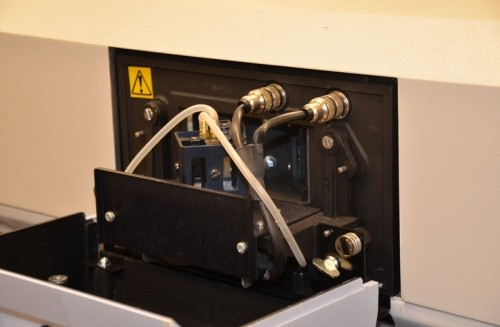
\includegraphics[scale=0.4]{figs/abertura.jpg}
	\caption{Compartimiento para colocar las muestras en un espectrómetro Perkin Elmer LS55 Luminsescence Spectrometer. \cite{PELS55}}
	\label{fig:abertura}
\end{figure}

\begin{figure}%[H]
	\centering
	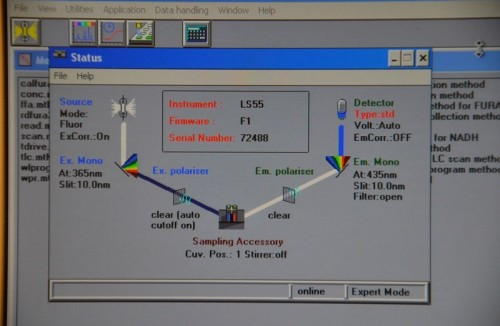
\includegraphics[scale=0.4]{figs/FL_Winlab.jpg}
	\caption{Software FL Winlab; para manejar el espectrómetro Perkin Elmer LS55. \cite{PELS55}}
	\label{fig:FL_Winlab}
\end{figure}

\begin{figure}%[H]
	\centering
	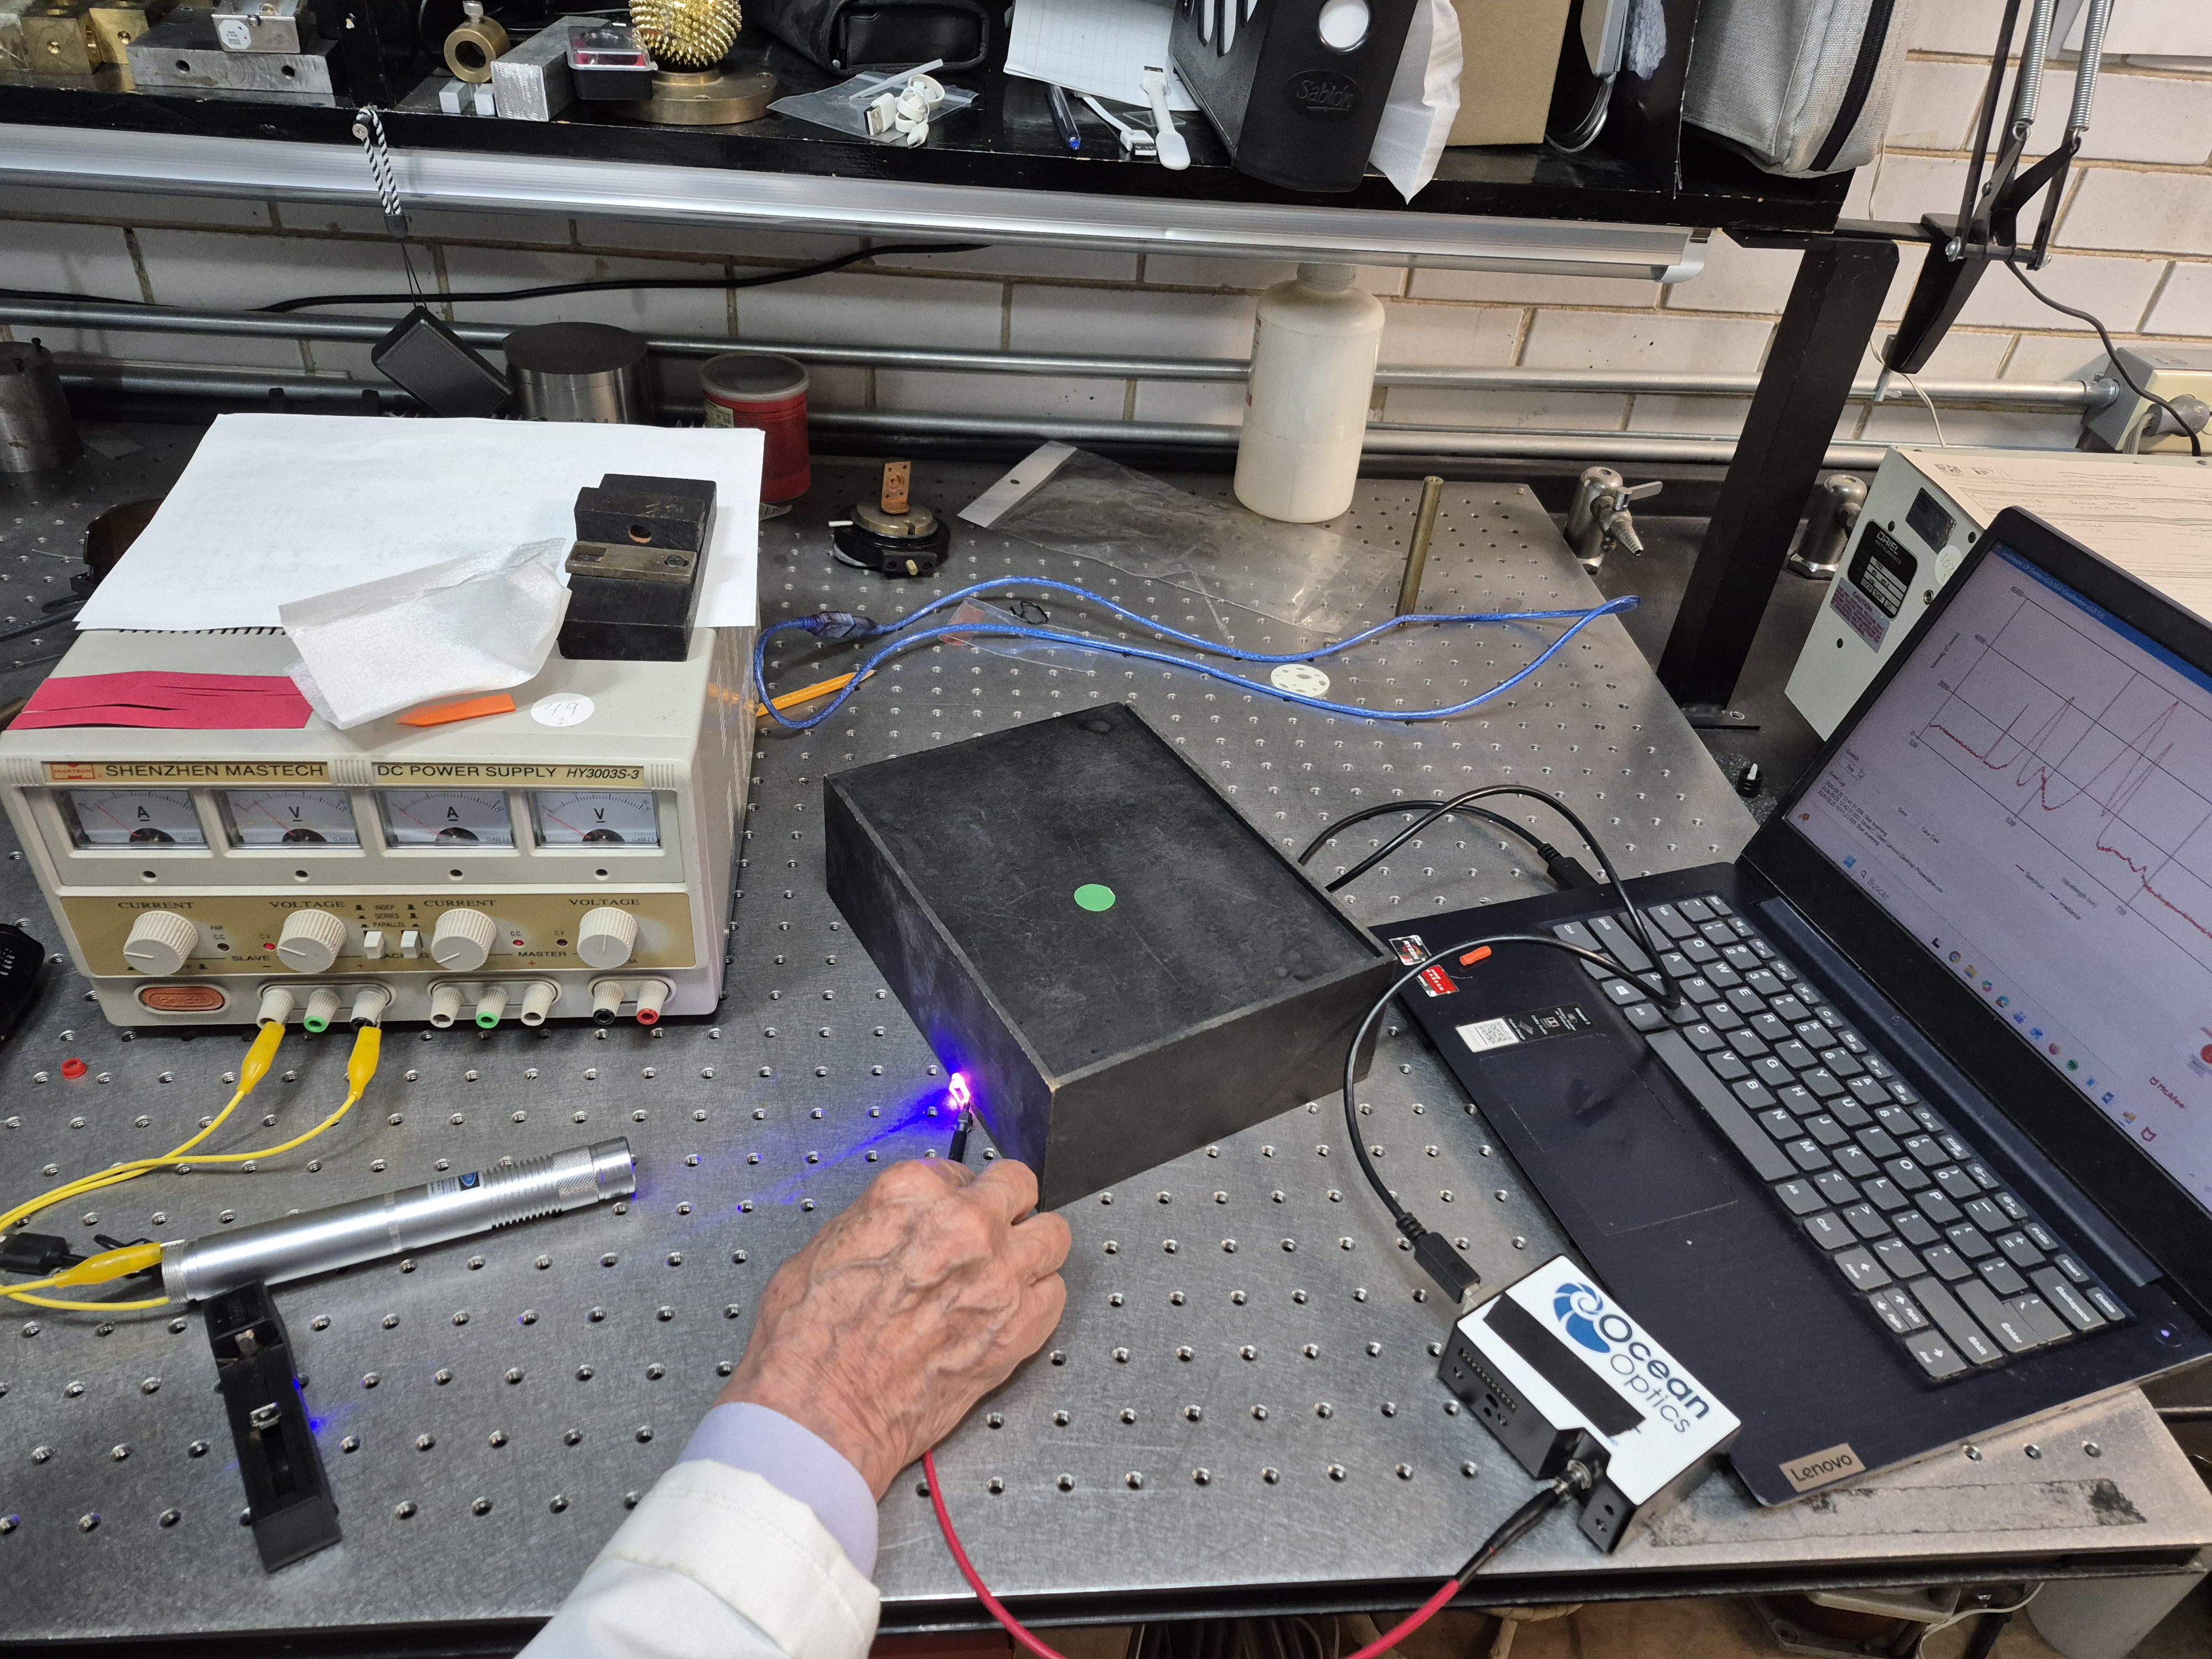
\includegraphics[scale=0.05]{figs/OceanOptics.jpg}
	\caption{Configuración manual de un láser y una fibra óptica para tomar espectros de emisión a través de un espectrómetro Ocean Optics.}
	\label{fig:OceanOptics}
\end{figure}

\noindent Se analizaron las siguientes siete muestras de tierras raras: un cristal mixto de fosfato y metafosfato de magnesio dopado con óxido de disprosio [Mg(PO$_3$)$_2$:Mg$_3$(PO$_4$)$_2$:Dy$_2$O$_3$ a una composición molar de $49.25\%$, $49.25\%$ y $1\%$, respectivamente], un cristal de niobato de litio dopado con óxido de disprosio [LiNbO$_3$:Dy$_2$O$_3$ a una composición molar de $99\%$ y $1.5\%$, respectivamente], un cristal de metafosfato de zinc dopado con óxido de disprosio [Zn(PO$_3$)$_2$:Dy$_2$O$_3$ a una composición molar de $99\%$ y $1\%$, respectivamente], un cristal mixto de fosfato y metafosfato de zinc dopado con óxido de samario [Zn(PO$_3$)$_2$:Zn$_3$(PO$_4$)$_2$:Sm$_2$O$_3$ a una composición molar de $49.5\%$, $49.5\%$ y $1\%$, respectivamente] un cristal de tetraborato de litio dopado con óxido de terbio [Li$_2$B$_4$O$_7$:Tb$_4$O$_7$, a una composición molar de $98\%$ y $2\%$, respectivamente], un cistal de metafosfato y ortofosfato de magnesio co-dopado con cloruro de estaño y óxido de europio [Mg(PO$_3$)$_2$:Mg$_3$(PO$_4$)$_2$:SnCl$_3$:Eu$_2$O$_3$, a una composición molar de $49\%$, $48\%$, $1\%$ y $3\%$, respectivamente] y un cistal de metafosfato y ortofosfato de zinc dopado con óxido de praseodimio [Zn(PO$_3$)$_2$:Zn$_3$(PO$_4$)$_2$:Pr$_2$O$_3$, a una composición molar de $49\%$, $49\%$ y $2\%$, respectivamente].

Primero se buscó en cada muestra la luz de excitación en la que se presentara el fenómeno de fotoluminiscencia; para ello, se utilizaron distintas lámparas de mano que emitían a una longitud de onda en específico, y se eligió la lámpara que mejor logró este efecto en el cristal. En el anexo (Figuras \ref{fig:Dy_Mg-fotos}-\ref{fig:Tb-fotos}) se muestran los cristales tanto a la intemperie como con el fenómeno de fotoluminiscencia, indicando el haz de excitación correspondiente.

Después se utilizó un espectrómetro de fluorescencia y luminiscencia Perkin Elmer LS55 (Figura \ref{fig:PerkinELmer}) para obtener el espectro de emisión de tres muestras: del disprocio en un fosfato y meta-fosfato de magnesio, el del samario y el del terbio. En la abertura del espectrómetro (Figura \ref{fig:abertura}) se colocó cada cristal y con un pedazo de papel (para ver la trayectoria del láser) se verificó que el haz incidiera sobre la mestra. Posteriormente se cerró este compartimiento y con el software FL Winlab (Figura \ref{fig:FL_Winlab}) se configuró el haz de excitación para cada muestra y se estableció que el recorrido del espectro fuera de los $420$ nm hasta los $850$ nm; se le dio en iniciar y se exportaron los datos del espectro de emisión (longitud de onda [nm] vs. intensidad).

Para el resto de las muestras se utilizó una configuración distinta ya que hubo problemas de comunicación entre el software FL Winlab y el espectrómetro. La nueva configuración se hizo manualmente (Figura \ref{fig:OceanOptics}); se usó una fuente de poder Shenzhen Mastech HY3003S-3 para potenciar el láser y un espectrómetro Ocean Optics con una fibra óptica para apuntar hacia el haz de emisión. Con el software OceanView se realizó la captura de los datos del espectro de emisión (longitud de onda [nm] vs. intensidad). Esta configuración se utilizó en las siguientes muestras: del disprosio en niobato de litio, del disprocio en metafosfato de zinc, el del samario (nuevamente, con el objetivo de realizar una comparación entre las dos configuraciones para obtener los espectros), el del europio y el del praseodimio.\\
\textcolor{black}{\section{Resultados y Análisis}}

{\subsection{Dy$^{3+}$ en un ambiente de fosfato de magnesio}
\noindent Se muestra a continuación el espectro de emisión del ion de disprosio en una matriz vítrea de fosfato de magnesio: 
\begin{figure}[H]
    \centering
    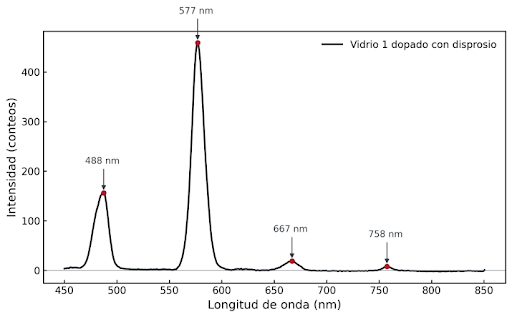
\includegraphics[scale=0.42]{disprosio_fosfato.png}
    \caption{Espectro de emisión del fosfato de magnesio dopado con un ion trivalente de disprosio}
    \label{fig:placeholder}
\end{figure}
Observamos que prresenta 4 máximos de intensidad localizados alrededor de $487.5\pm 16$ nm, $577\pm 14$ nm, $667 \pm 16$ nm, $758 \pm 9$ nm. Las bandas de mayor intensidad se presentan en $488 \pm 8$ nm que corresponde al color azul y $577\pm 14$ nm que corresponde al color amarillo. Mientras que las bandas de menor intensidad se observan en $667 \pm 16$ nm y $758 \pm 9$ nm. A partir de estas longitudes de onda, se calcularon los números de onda correspondientes mediante

\begin{equation}
    \tilde{\nu} = \frac{10^{7}}{\lambda}
\label{eq:numero_onda}
\end{equation}

obteniéndose $(20513 \pm 1348)\,\text{cm}^{-1}$, $(17331 \pm 841)\,\text{cm}^{-1}$, $(14993 \pm 742)\,\text{cm}^{-1}$, $(13201 \pm 314)\,\text{cm}^{-1}$. Estos valores están asociados a las diferencia de energía observadas. A continuación, se muestra un gráfico de la energía asociada a cada longitud de onda: 
\begin{figure}[H]
    \centering
    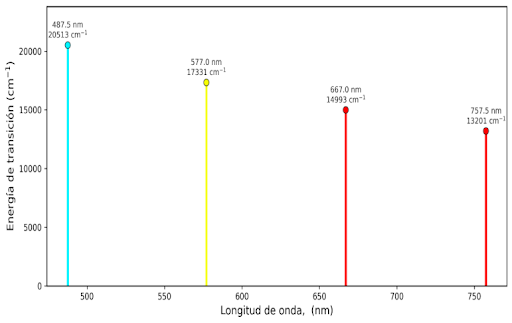
\includegraphics[scale=0.45]{figs/niv_energia_fosfato_magnesio.png}
    \caption{Energías asociadas a las diferencias de energía entre niveles. Se observa la energía correspondiente a cada longitud de onda}
    \label{fig:placeholder}
\end{figure}
El máximo de menor longitud de onda observado en el espectro de emisión está asociado a una mayor energía, mientras que el máximo de mayor longitud de onda corresponde a una menor energía de transición entre niveles. El diagrama de niveles para el ion de disprosio en fosfato de magnesio muestra transiciones radiativas desde el nivek $^4F_{9/2}$ del ion Dy$^{3+}$ hacia niveles de menor energía. La transición de menor longitud de onda, $(488 \pm 8)\,\text{nm}$ , termina en el estado fundamental  $^6H_{15/2}$ y corresponde a la mayor energía de emisión  $(20513 \pm 1347)\,\text{cm}^{-1}$. Las transiciones de asociadas a luz registrada para las longitudes de onda restantes terminan en niveles más altos t energías menores. Esto corresponde a la relación inversa entre la longitud de onda de la radiación y su energía.
\begin{figure}[H]
    \centering
    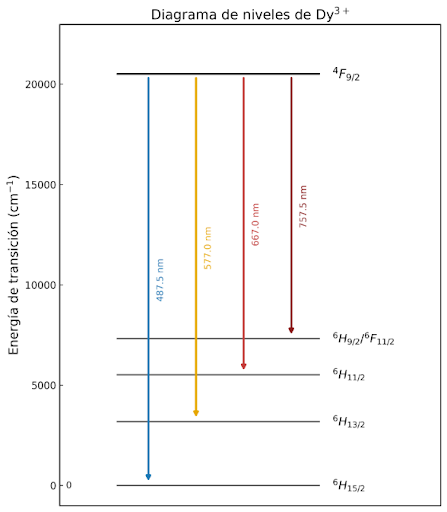
\includegraphics[scale=0.45]{figs/diagrama de niveles.png}
    \caption{Niveles de transición del Dy$^{3+}$}
    \label{fig:placeholder}
\end{figure}
{\subsection{Disprosio en un cristal de metafosfato de magnesio}
\begin{figure}[ht]
  \centering
  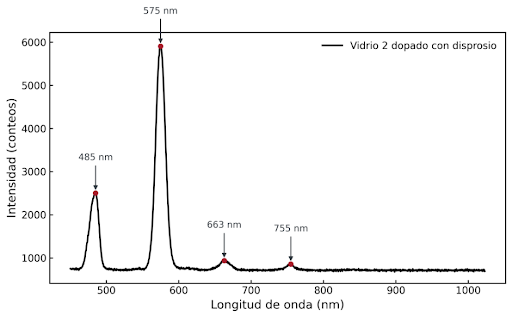
\includegraphics[scale=0.45]{disprosio_metafosfato.png}

  \medskip

  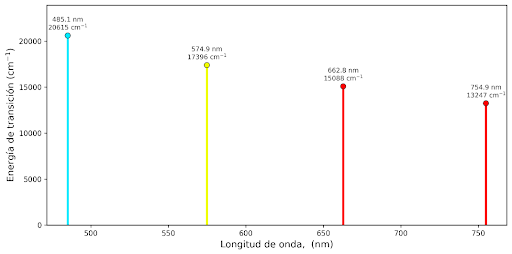
\includegraphics[scale=0.45]{energias_metafosfatos_2.png}
  \caption{Espectro de emisión del disprosio incorporado en metafosfato (Vidrio de metafosfato de zinc, Zn(PO$_3$)$_2$, dopado con óxido de disprosio (Dy$_2$O$_3$) al 1\%.) de magnesio y energía asociadas a cada longitud de onda detectada}
\end{figure}
El espectro de emisión presenta 4 bandas procipales, con máximos en $485. 1\pm 9.2\,\text{nm}$, $574.9\pm 10\,\text{nm}$, $662.8\pm 10\,\text{nm}$, $754.9\pm 9\,\text{nm}$. La banda centrada en $574.9\pm 10\,\text{nm}$ presenta la mayor intensidad, alrededor de 5900 cuentas. Se puede observar que la  emisión más intensa está localizada en la región del amarillo y se asocia a la transición de $^4F_{9/2}\rightarrow{}^6H_{13/2}$ del ion $Dy^{3+}$. Las demás bandas se deben a transiciones del nivel $^4F_{9/2}$ a niveles de menor energía. A continuación se muestra el diagrama de niveles de energía: 
\begin{figure}[H]
    \centering
    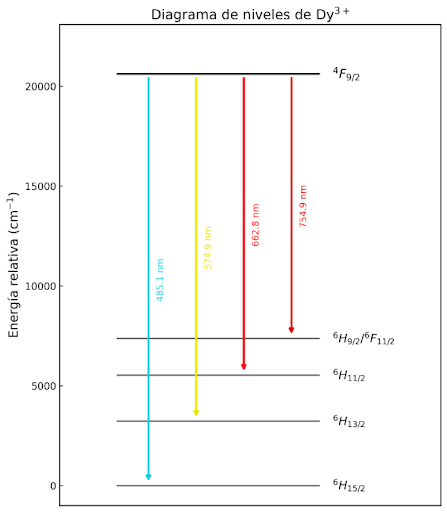
\includegraphics[scale=0.45]{figs/disgramas_metafosfato.png}
    \caption{Diagrama de niveles de Dy$_2$O$_3$) al 1\% en un vidrio de metafosfato de zinc, Zn(PO$_3$)$_2$}
    \label{fig:placeholder}
\end{figure}
 
Al comparar los espectros de emisión del ion de disprosio en los distintos ambientes, tenemos lo siguiente: 
\begin{figure}[H]
    \centering
    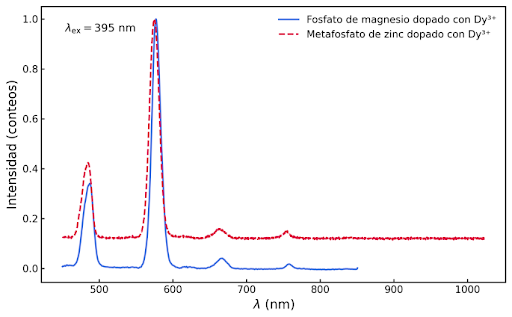
\includegraphics[scale=0.45]{figs/dos_espectros.png}
    \caption{Comparación de los dos espectros de emisión obtenidos a partir del ion de disprosio en distintos ambientes}
    \label{fig:placeholder}
\end{figure}

Las diferencias observadas pueden relacionarse con el ambiente químico que proporciona cada matriz al ion Dy$^{3+}$.

{\subsection{Samario en un ambiente de fosfato de zinc}
\noindent 
El espectro de emisión del vidrio de fosfato de zinc dopado con Sm$_2$O$_3$
presenta cuatro bandas principales, con máximos aproximados en $566.0 \pm 13.5$, $602.5 \pm 14$,
$648 \pm 14$ y $708\pm 20\,\text{nm}$. La banda de 602\,\text{nm} es la más intensa,
con un máximo cercano a 185 cuentas. Las bandas de $648 \pm 14$ y  $566.0 \pm 13.5 $\,\text{nm}
alcanzan intensidades aproximadas de 110 y 70 cuentas, respectivamente,
mientras que la banda de $708.5\pm 20.5$\,\text{nm} es débil, con una intensidad
cercana a 7 cuentas.

\begin{figure}[ht]
  \centering
  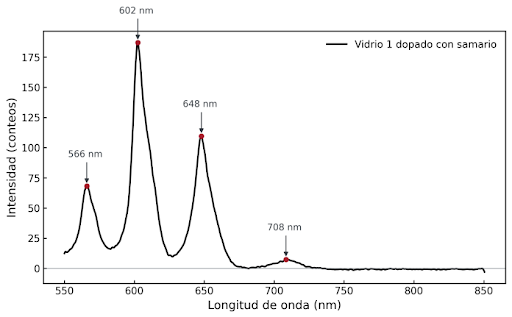
\includegraphics[scale=0.45]{figs/samario_espectro.png}

  \medskip

  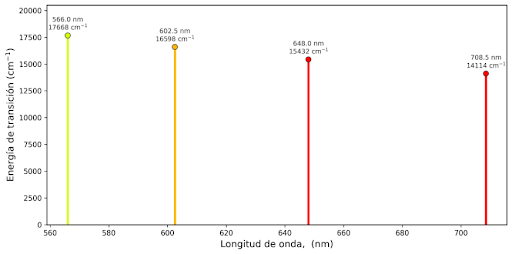
\includegraphics[scale=0.45]{figs/energia_samario_1.png}
  \caption{Espectro de emisión del vidrio de fosfato de zinc,
Zn(PO$_3$)$_2$:Zn$_3$(PO$_4$)$_2$, dopado con óxido de samario
(Sm$_2$O$_3$), y energías asociadas a las longitudes de onda detectadas.}
\end{figure}
El espectro de emisión del vidrio de fosfato de zinc dopado con Sm$_2$O$_3$
presenta bandas en $566.0 \pm 13$ , $602.5 \pm 14$, $648.0 \pm 14 $ y $708.5 \pm 20.5\,\text{nm}$. La banda de
$602.5\,\text{nm}$ es la más intensa y la de $708.5\,\text{nm}$, la menos
intensa. Los números de onda correspondientes son $17668\pm 843.3 $, $16598\pm 771.7$, $15432\pm 667$ y $14114\pm  817\,\text{cm}^{-1}$, respectivamente. Las emisiones se asignan a transiciones desde $^4G_{5/2}$ hacia los niveles $^6H_{5/2}$, $^6H_{7/2}$, $^6H_{9/2}$ y $^6H_{11/2}$ del Sm$^{3+}$.
\begin{figure}[H]
    \centering
    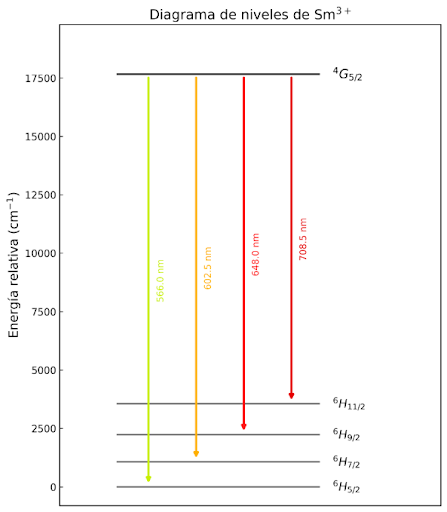
\includegraphics[scale=0.45]{figs/diagrama de niveles_samario.png}
    \caption{Diagrama de niveles para Sm$_2$O$_3$ en un ambiente de vidrio de fosfato de zinc (Zn(PO$_3$)$_2$:Zn$_3$(PO$_4$)$_2$) }
    \label{fig:placeholder}
\end{figure}
{\subsection{Samario en un ambiente de fosfato de zinc - medidas con un segundo aparato de medición}
\begin{figure}[ht]
  \centering
  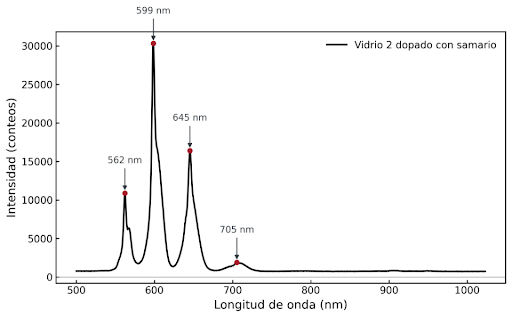
\includegraphics[scale=0.45]{figs/espectro_samario_2.png}

  \medskip

  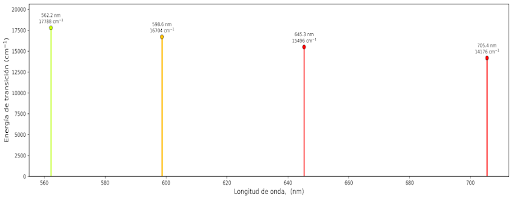
\includegraphics[scale=0.45]{figs/samario_energias_aparato_2.png}
  \caption{Espectro de emisión del vidrio de fosfato de zinc,
Zn(PO$_3$)$_2$:Zn$_3$(PO$_4$)$_2$, dopado con óxido de samario
(Sm$_2$O$_3$), y energías asociadas a las longitudes de onda detectadas (con un segundo aparato de medición).}
\end{figure}
El espectro obtenido con el espectrómetro \textit{Ocean Optics}  presenta bandas alrededor
de $562.2\pm 9.5$, $598.6\pm 0.3$, $645\pm 0.3$ y $705.4\pm 41.2\ ,\text{nm}$, asignadas a transiciones del Sm$^{3+}$
desde $^4G_{5/2}$ hacia $^6H_{5/2}$, $^6H_{7/2}$, $^6H_{9/2}$ y
$^6H_{11/2}$, respectivamente. Estas posiciones son cercanas a las del
primer aparato, en concordancia con la
medición del mismo material. Las pequeñas diferencias pueden relacionarse
con la resolución o calibración de los equipos. La banda cercana a
$598.6\pm 0.3 \,\text{nm}$ es la más intensa en esta medición; las intensidades
absolutas no se comparan directamente entre aparatos porque pueden
depender de sus condiciones de detección. Los números de onda calculados
son aproximadamente $17788\pm 602$, $16704\pm 19.6 $, $15496\pm 16.3 $ y $14176\pm 1664 \,\text{cm}^{-1}$.
%%%%% TERBIO %%%%%%%%%%%%%%%%%%%%%%%%%%%%%%%%%%%%%%%%%%%%%%

{\subsection{Terbio en un cristal de tetraborato de litio}
\noindent En la Figura \ref{fig:Tb_espectro} se muestra su espectro de emisión. Se consideraron como bandas de mayor intensidad a las intensidades máximas de la gráfica más una incertidumbre, calculada como el ancho de la mitad de la intensidad máxima correspondiente. Por tanto, se obtuvieron los siguientes valores: $\lambda_{Tb_1} = 492.0 \pm 18.00$ nm, $\lambda_{Tb_2} = 547.5 \pm 11.50$ nm, $\lambda_{Tb_3} = 590.0 \pm 16.50$ nm y $\lambda_{Tb_4} = 625.5 \pm 12.50$ nm.

\begin{figure}%[H]
    \centering
    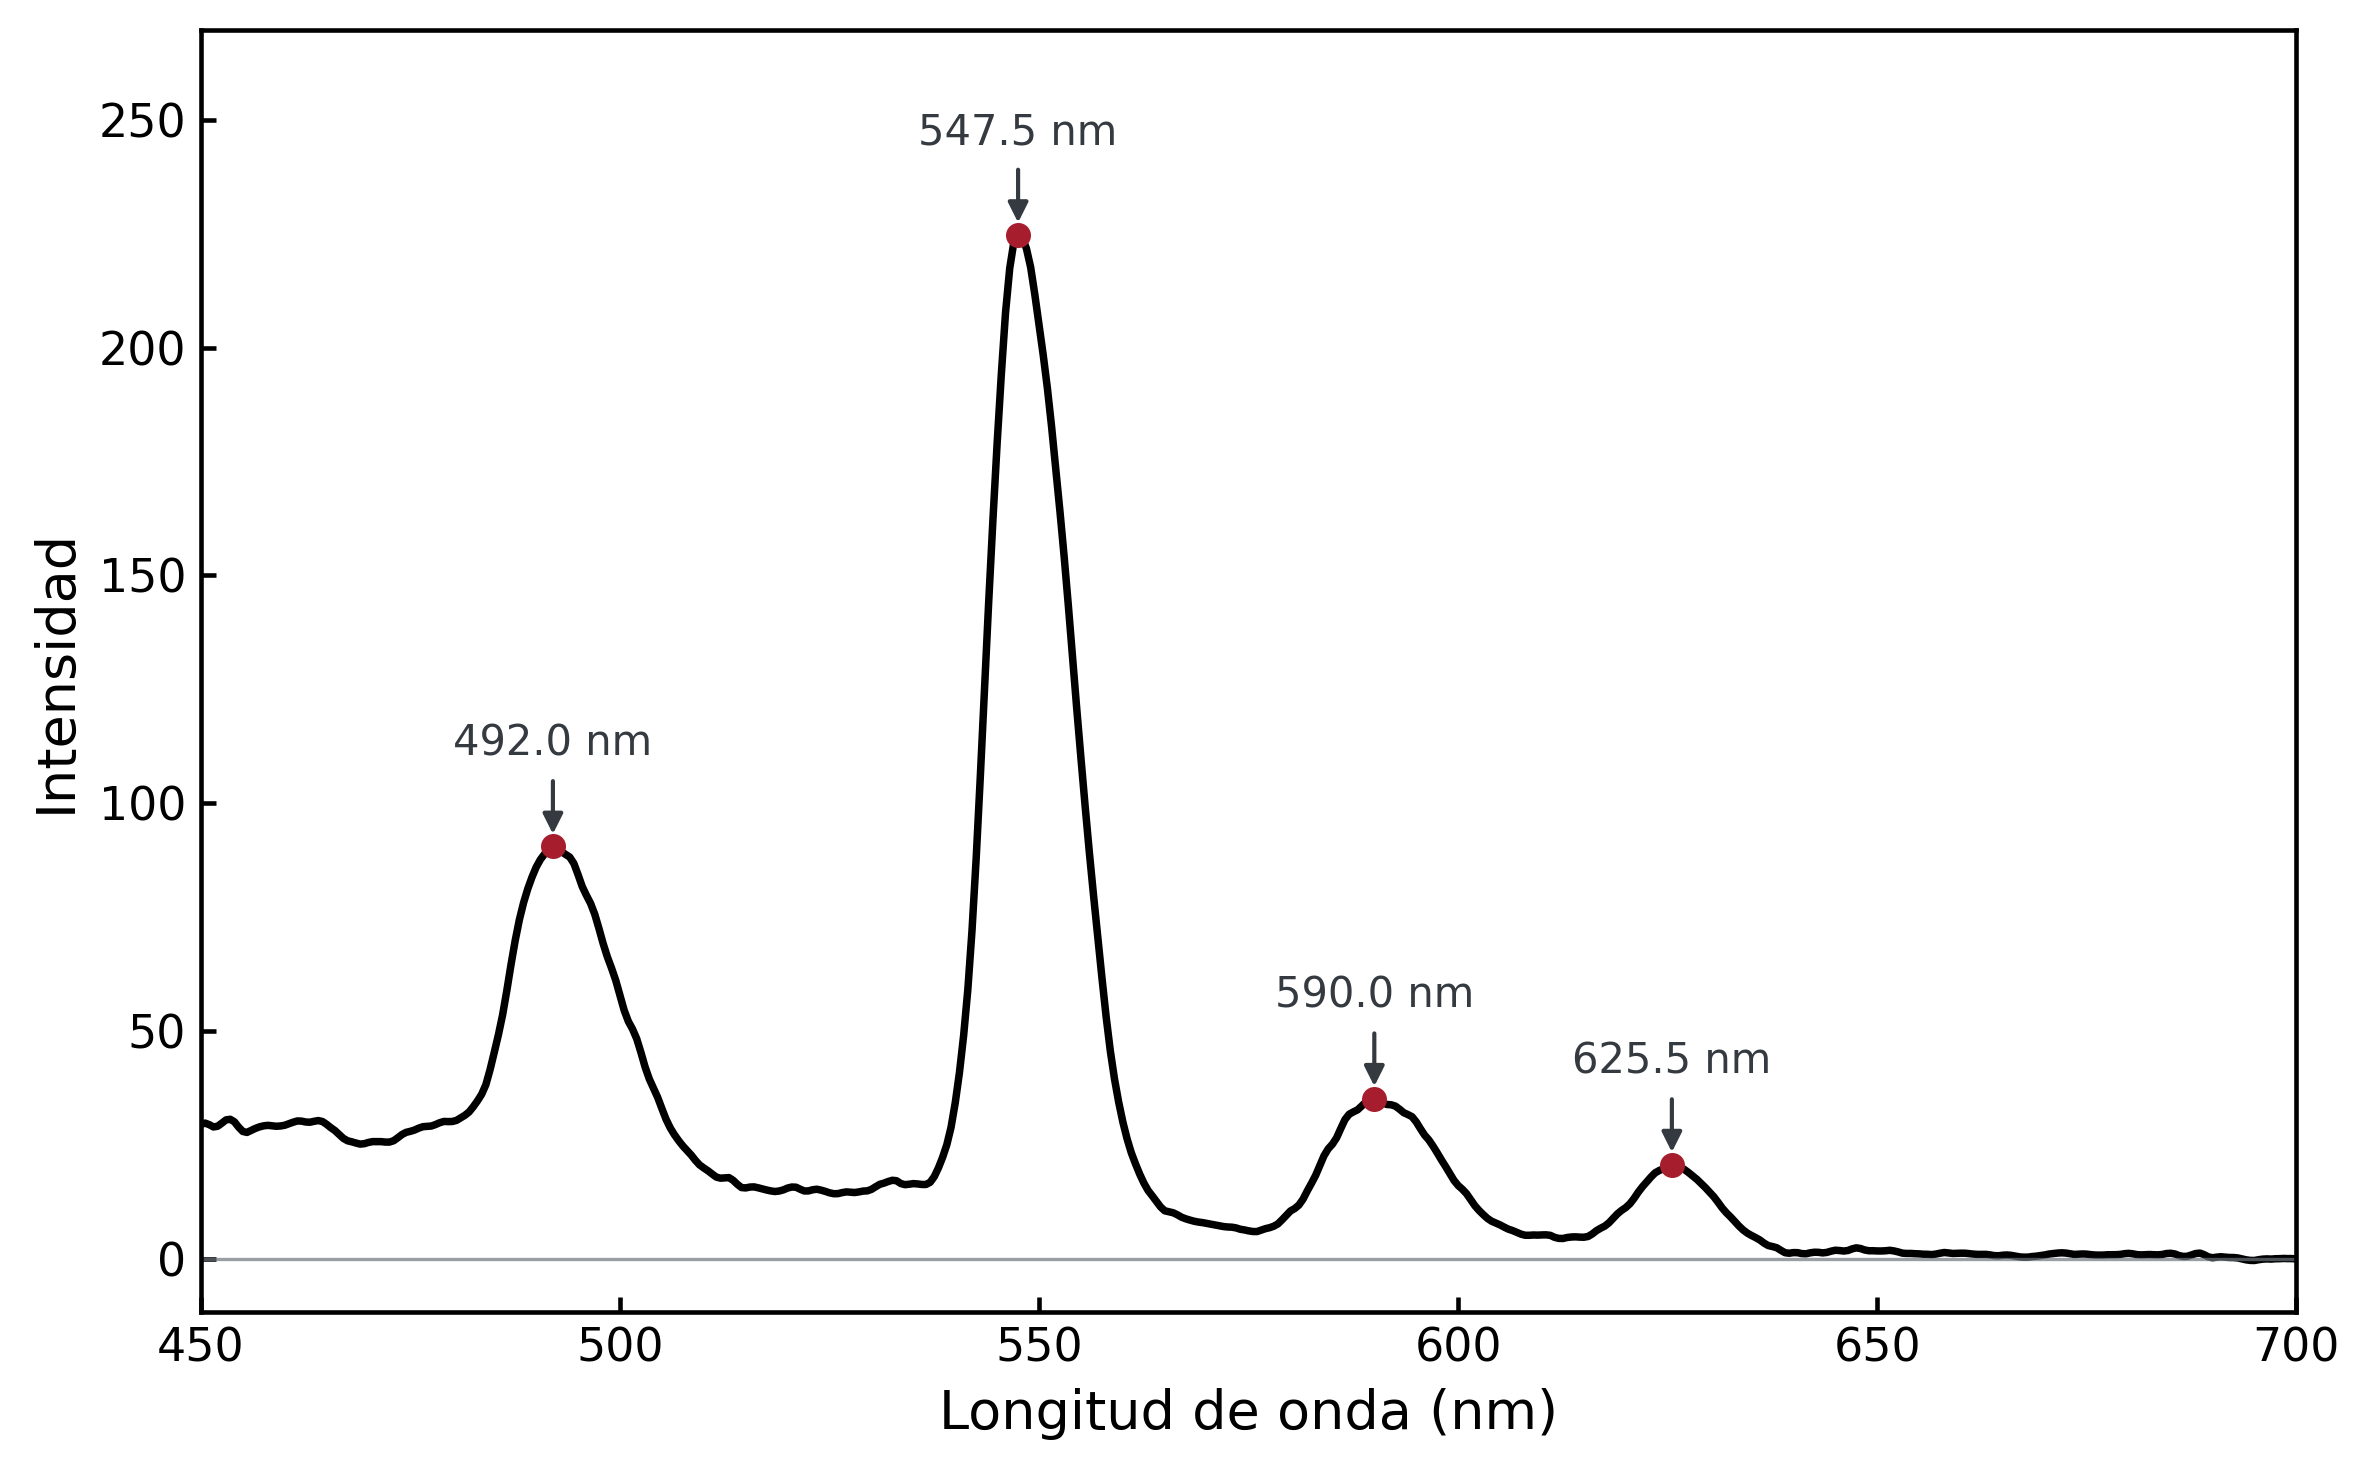
\includegraphics[scale=0.1]{figs/Tb_espec.png}
    \caption{Espectro de emisión de un cristal de Li$_2$B$_4$O$_7$ ($98\%$, composición molar) dopado con Tb$_4$O$_7$ ($2\%$). Se señalan las intensidades máximas.}
    \label{fig:Tb_espectro}
\end{figure}

Se utilizó la Ecuación \ref{eq:numero_onda} y se
calcularon las siguientes energías: $E_{Tb_1} = 20325.20
\pm 1489.20\ \mathrm{cm}^{-1}$, $E_{Tb_2} = 18264.84
\pm 767.63\ \mathrm{cm}^{-1}$, $E_{Tb_3} = 116949.15
\pm 948.75\ \mathrm{cm}^{-1}$ y $E_{Tb_4} = 15987.21
\pm 639.23\ \mathrm{cm}^{-1}$. Finalmente, para
la elaboración del diagrama de energía de este ion (Figura
\ref{fig:Tb_diagrama-ener}) se consideraron el rango de
las incertidumbres de la energía, y se eligió el que mejor
correspondía con la información disponible
actualmente. \cite{Tb-literatura}

\begin{figure}%[H]
    \centering
    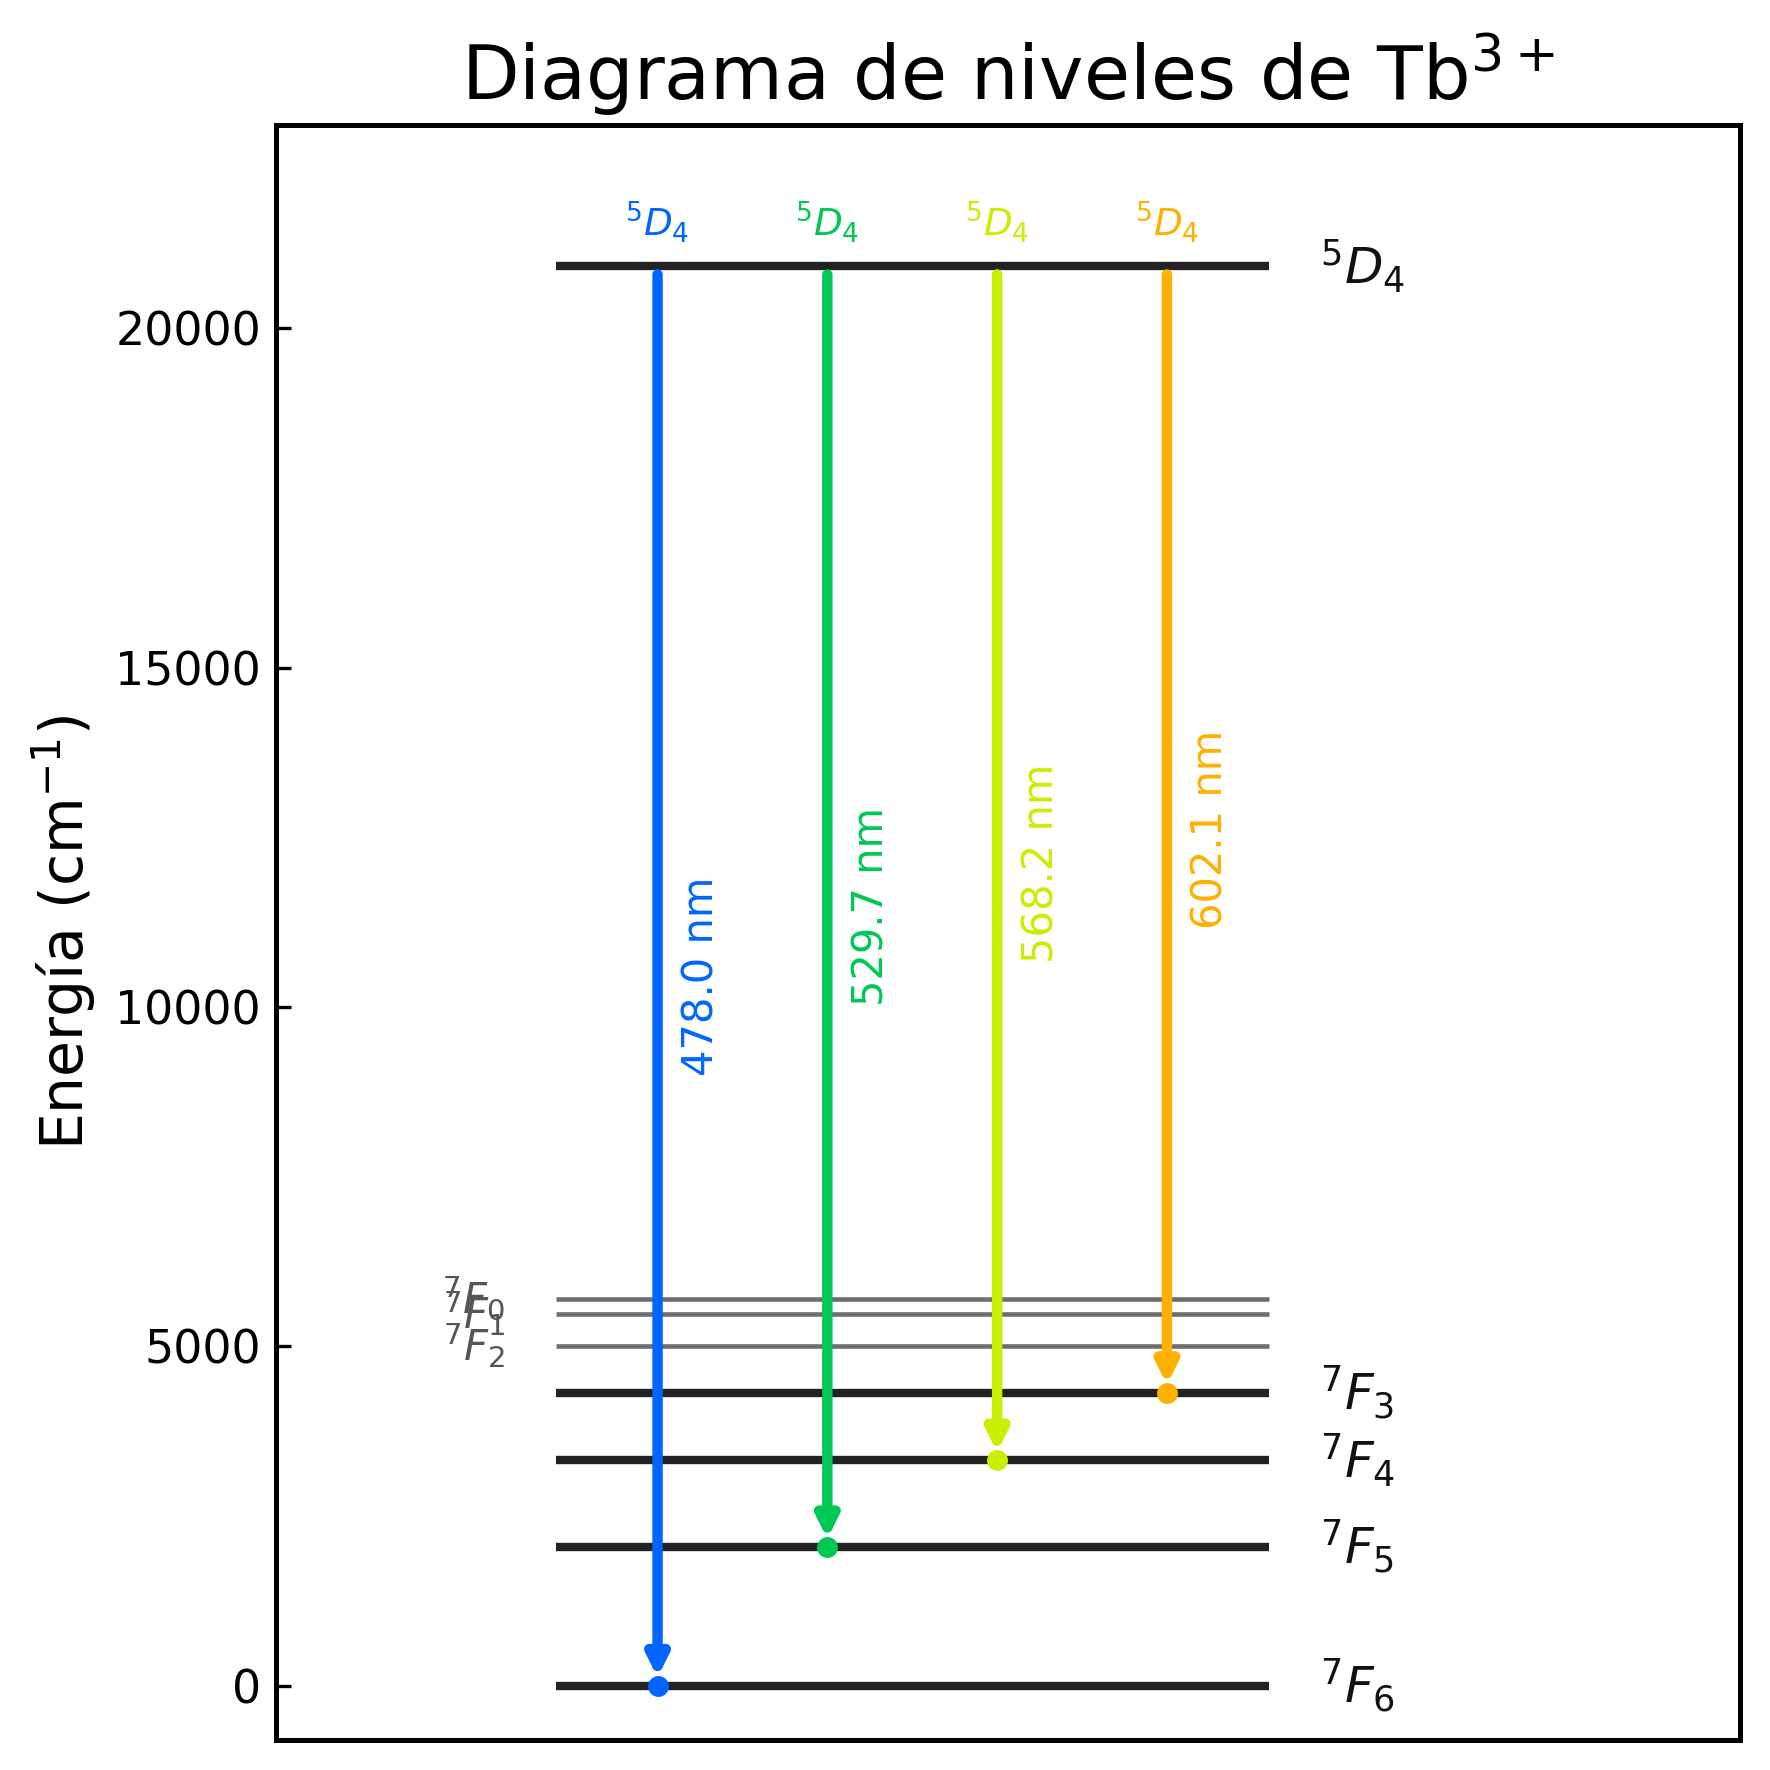
\includegraphics[scale=0.11]{figs/Tb-diag_ener.png}
    \caption{Diagrama de los niveles de energía de transición (fotoluminiscencia) del $Tb^{3+}$ calculado a partir de las intesidades máximas del espectro de emisión de un cristal de Li$_2$B$_4$O$_7$ ($98\%$, composición molar) dopado con Tb$_4$O$_7$ ($2\%$). Se señalan las longitudes de onda correspondientes.}
    \label{fig:Tb_diagrama-ener}
\end{figure}

%%%%% EUROPIO %%%%%%%%%%%%%%%%%%%%%%%%%%%%%%%%%%%%%%%%%%%%%

{\subsection{Europio en un cristal de metafosfato y ortofosfato de magnesio con cloruro de estaño}
\noindent En la Figura \ref{fig:Eu_espectro} se muestra su espectro de emisión. Se consideraron como bandas de mayor intensidad a las intensidades máximas de la gráfica más una incertidumbre, calculada como el ancho de la mitad de la intensidad máxima correspondiente. Por tanto, se obtuvieron los siguientes valores: $\lambda_{Eu_1} = 611.52 \pm 5.21$ nm, $\lambda_{Eu_2} = 592.02 \pm 13.28$ nm, $\lambda_{Eu_3} = 701.71 \pm 7.40$ nm y $\lambda_{Eu_4} = 653.22 \pm 24.62$ nm.

\begin{figure}%[H]
    \centering
    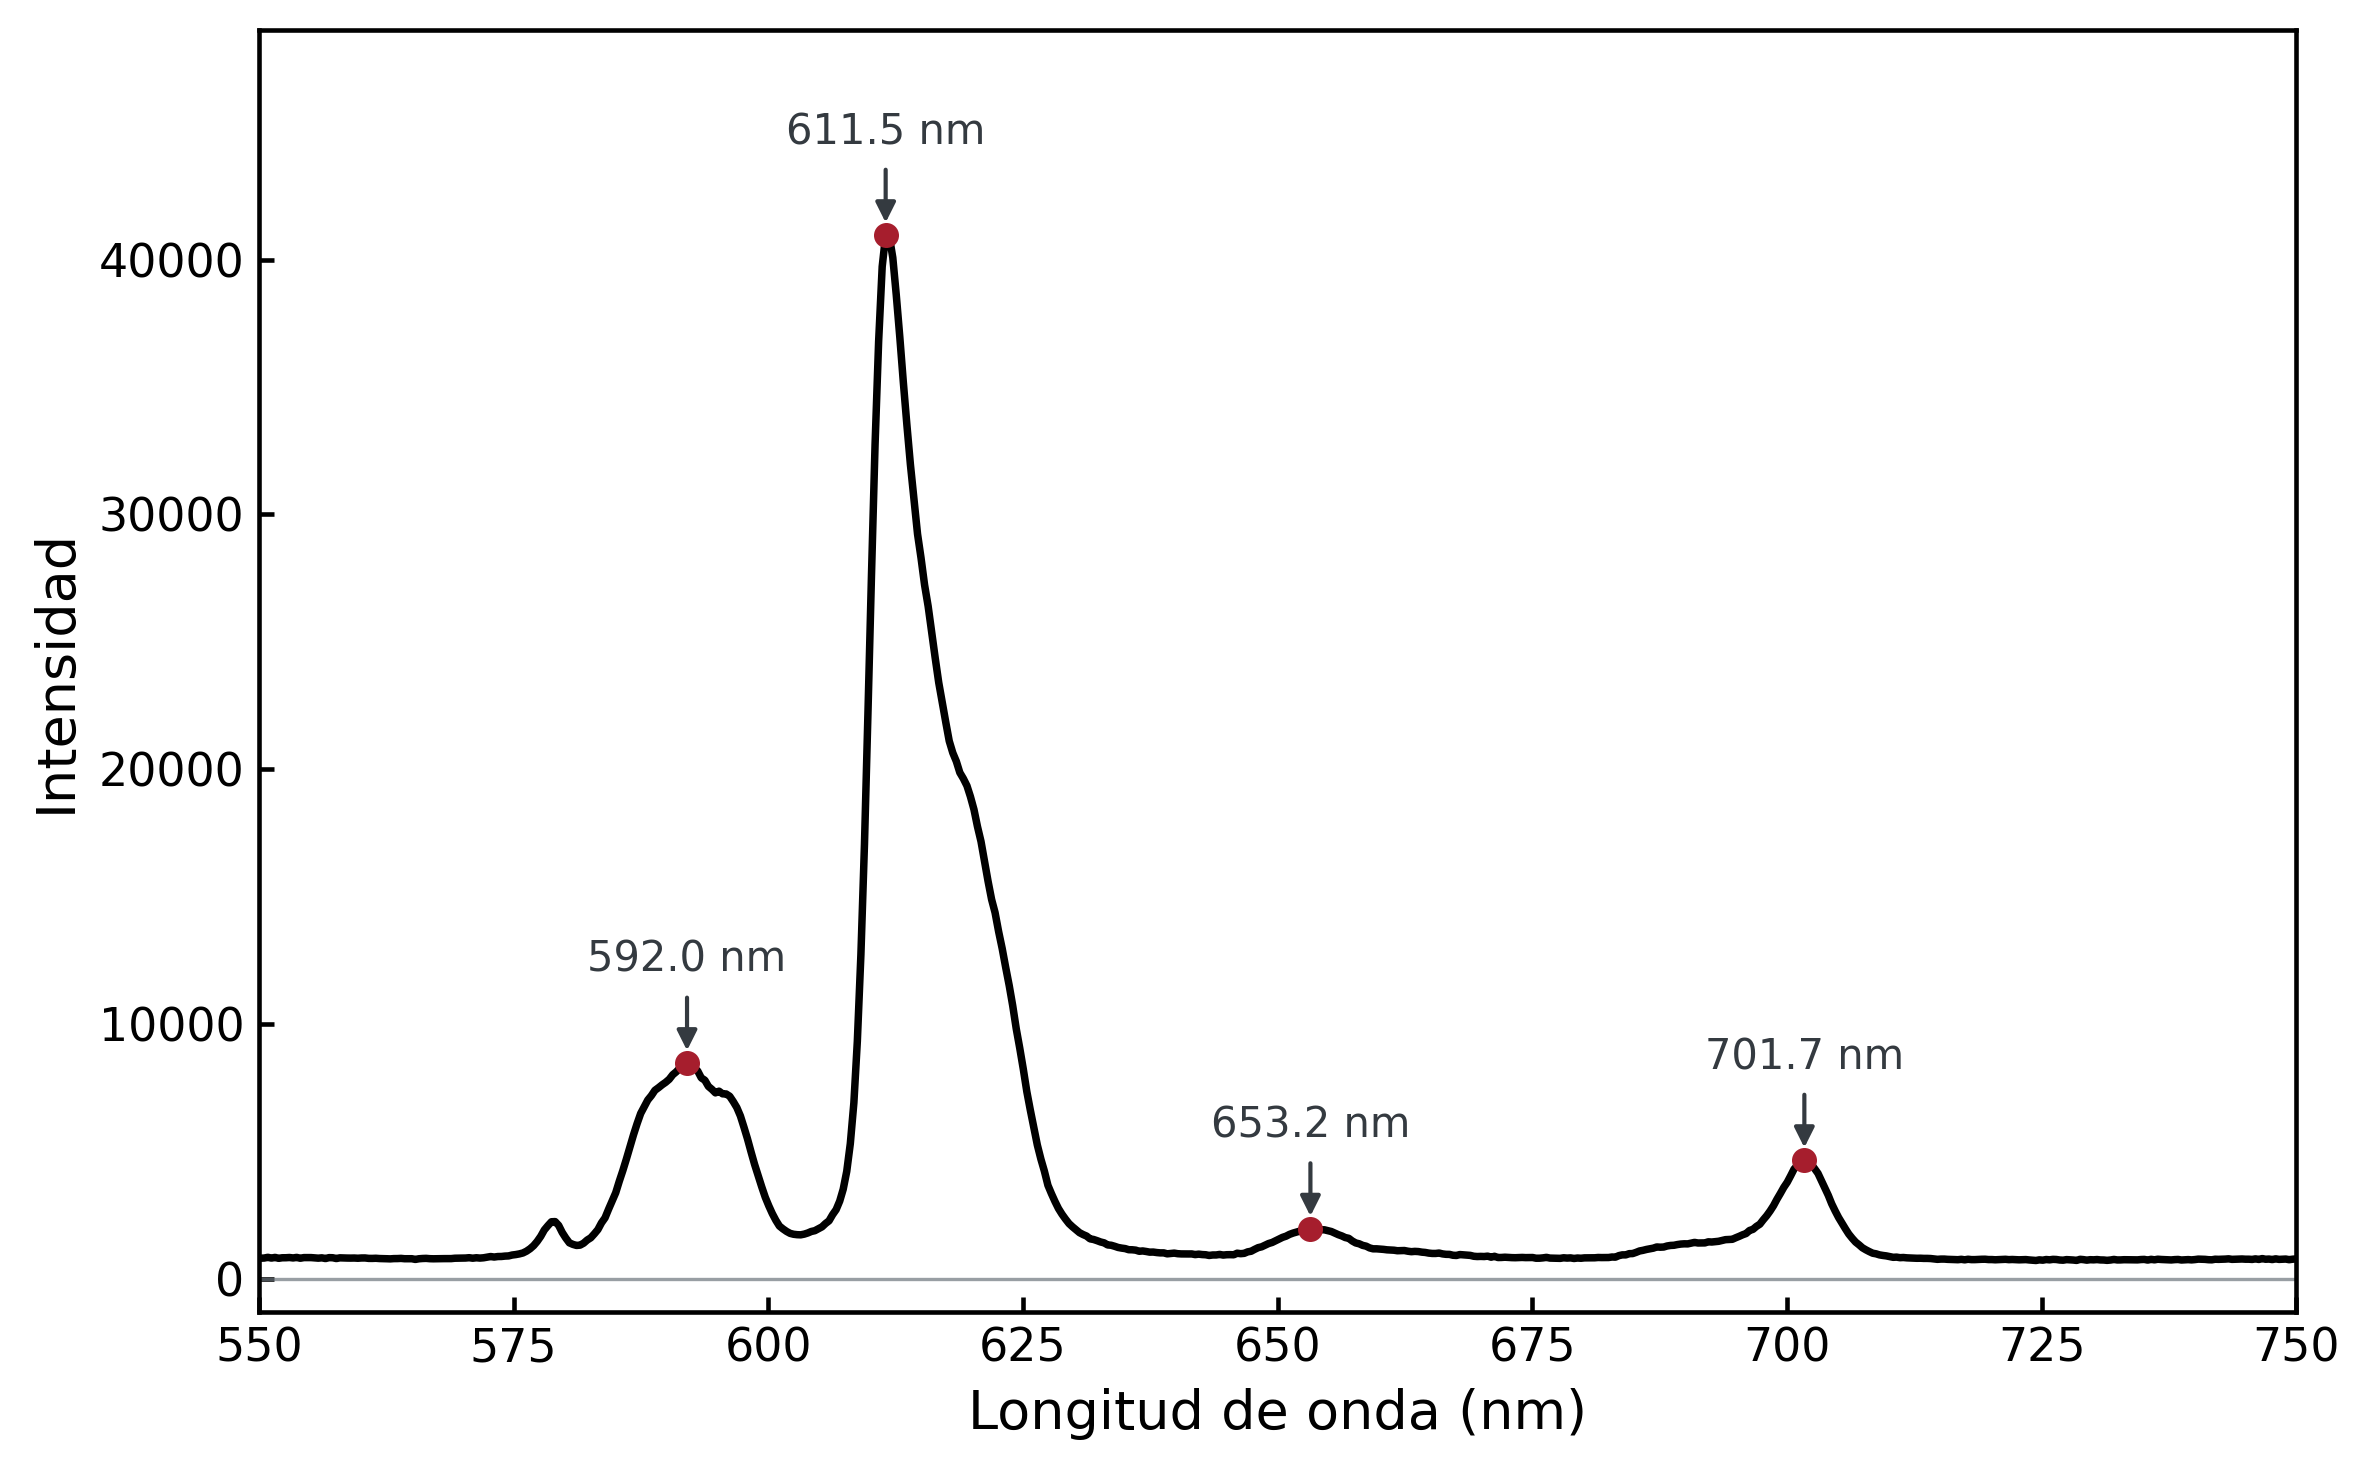
\includegraphics[scale=0.1]{figs/Eu-espec.png}
    \caption{Espectro de emisión de un cristal de Mg(PO$_3$)$_2$:Mg$_3$(PO$_4$)$_2$:SnCl$_3$ ($49\%$, $48\%$, $1\%$, composición molar) dopado con Eu$_2$O$_3$ ($3\%$). Se señalan las intensidades máximas.}
    \label{fig:Eu_espectro}
\end{figure}

Se utilizó la Ecuación \ref{eq:numero_onda} y se
calcularon las siguientes energías: $E_{Eu_1} = 16352.69
\pm 278.66\ \mathrm{cm}^{-1}$, $E_{Eu_2} = 16891.32
\pm 758.18\ \mathrm{cm}^{-1}$, $E_{Eu_3} = 14250.90
\pm 300.60\ \mathrm{cm}^{-1}$ y $E_{Eu_4} = 15308.78
\pm 1155.62\ \mathrm{cm}^{-1}$. Finalmente,
para la elaboración del diagrama de energía de este ión
(Figura \ref{fig:Eu_diagrama-ener}) se consideraron el
rango de las incertidumbres de la energía, y se eligió el
que mejor correspondía con la información disponible
actualmente. \cite{Eu_Pr-literatura}

\begin{figure}%[H]
    \centering
    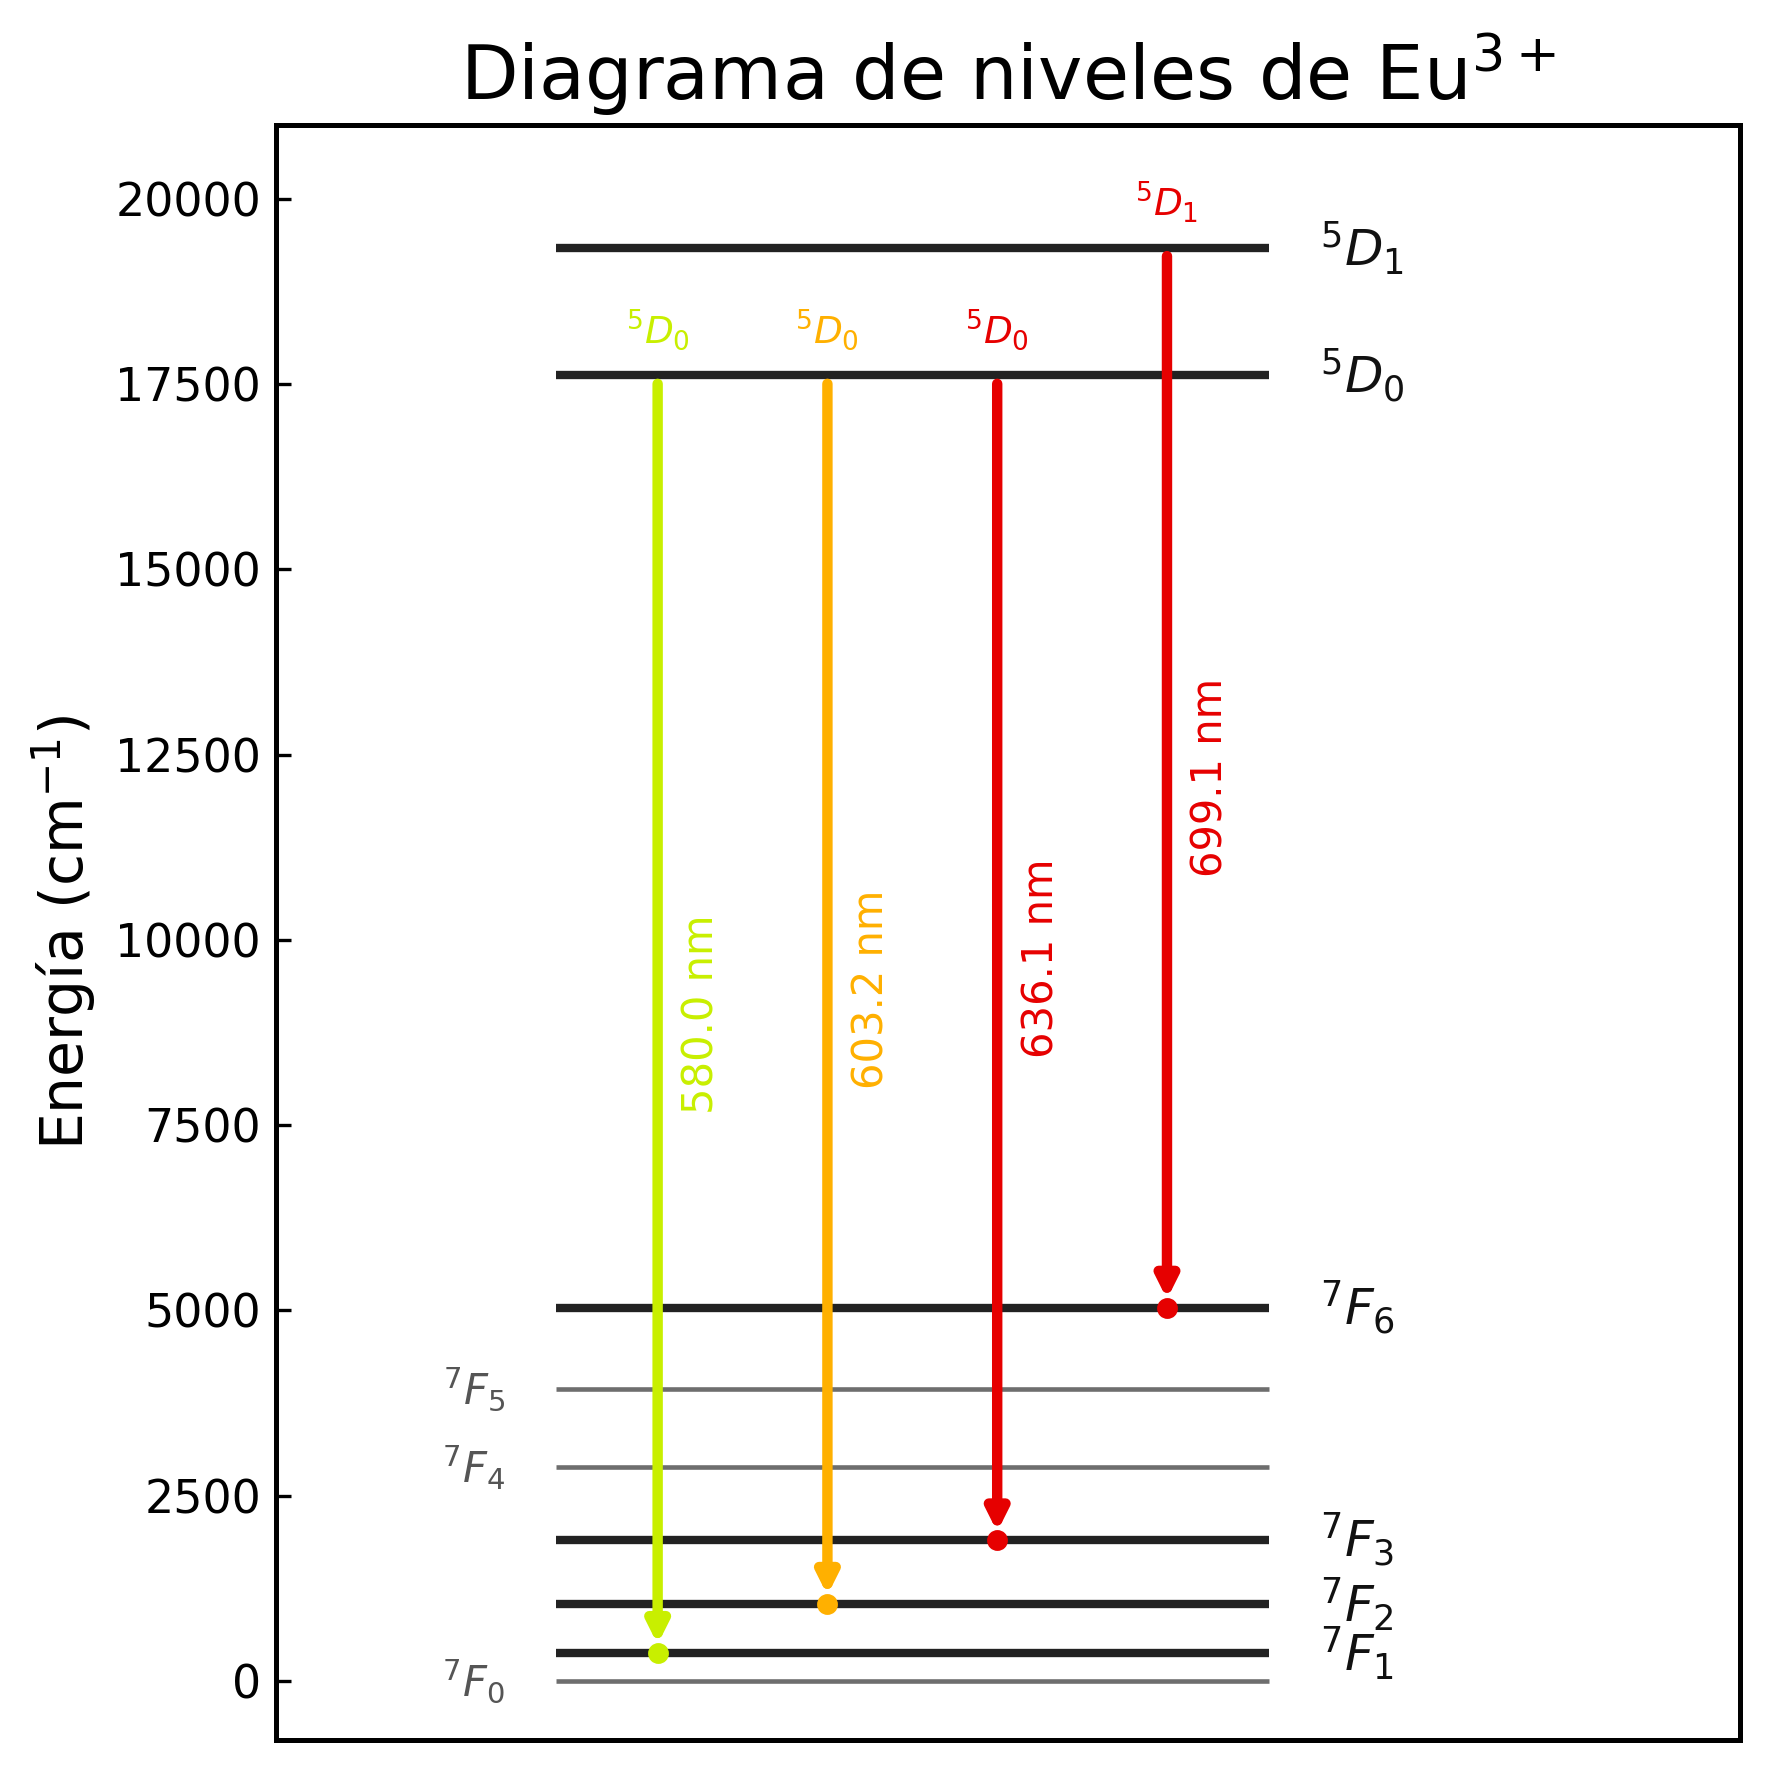
\includegraphics[scale=0.11]{figs/Eu-diag_ener.png}
    \caption{Diagrama de los niveles de energía de transición (fotoluminiscencia) del $Eu^{3+}$ calculado a partir de las intesidades máximas del espectro de emisión de un cristal de Mg(PO$_3$)$_2$:Mg$_3$(PO$_4$)$_2$:SnCl$_3$ ($49\%$, $48\%$, $1\%$, composición molar) dopado con Eu$_2$O$_3$ ($3\%$). Se señalan las longitudes de onda correspondientes.}
    \label{fig:Eu_diagrama-ener}
\end{figure}

%%%%% PRADEODIMIO %%%%%%%%%%%%%%%%%%%%%%%%%%%%%%%%%%%%%%%%%

{\subsection{Praseodimio en un cristal de metafosfato y ortofosfato de zinc}
\noindent En la Figura \ref{fig:Pr_espectro} se muestra su espectro de emisión. Se consideraron como bandas de mayor intensidad a las intensidades máximas de la gráfica más una incertidumbre, calculada como el ancho de la mitad de la intensidad máxima correspondiente. Por tanto, se obtuvieron los siguientes valores: $\lambda_{Pr_1} = 609.44 \pm 23.96$ nm, $\lambda_{Pr_2} = 640.88 \pm 8.59$ nm, $\lambda_{Pr_3} = 490.49 \pm 18.02$ nm, $\lambda_{Pr_4} = 525.64 \pm 30.25$ nm y $\lambda_{Pr_5} = 723.12 \pm 1.00$ nm.

\begin{figure}%[H]
    \centering
    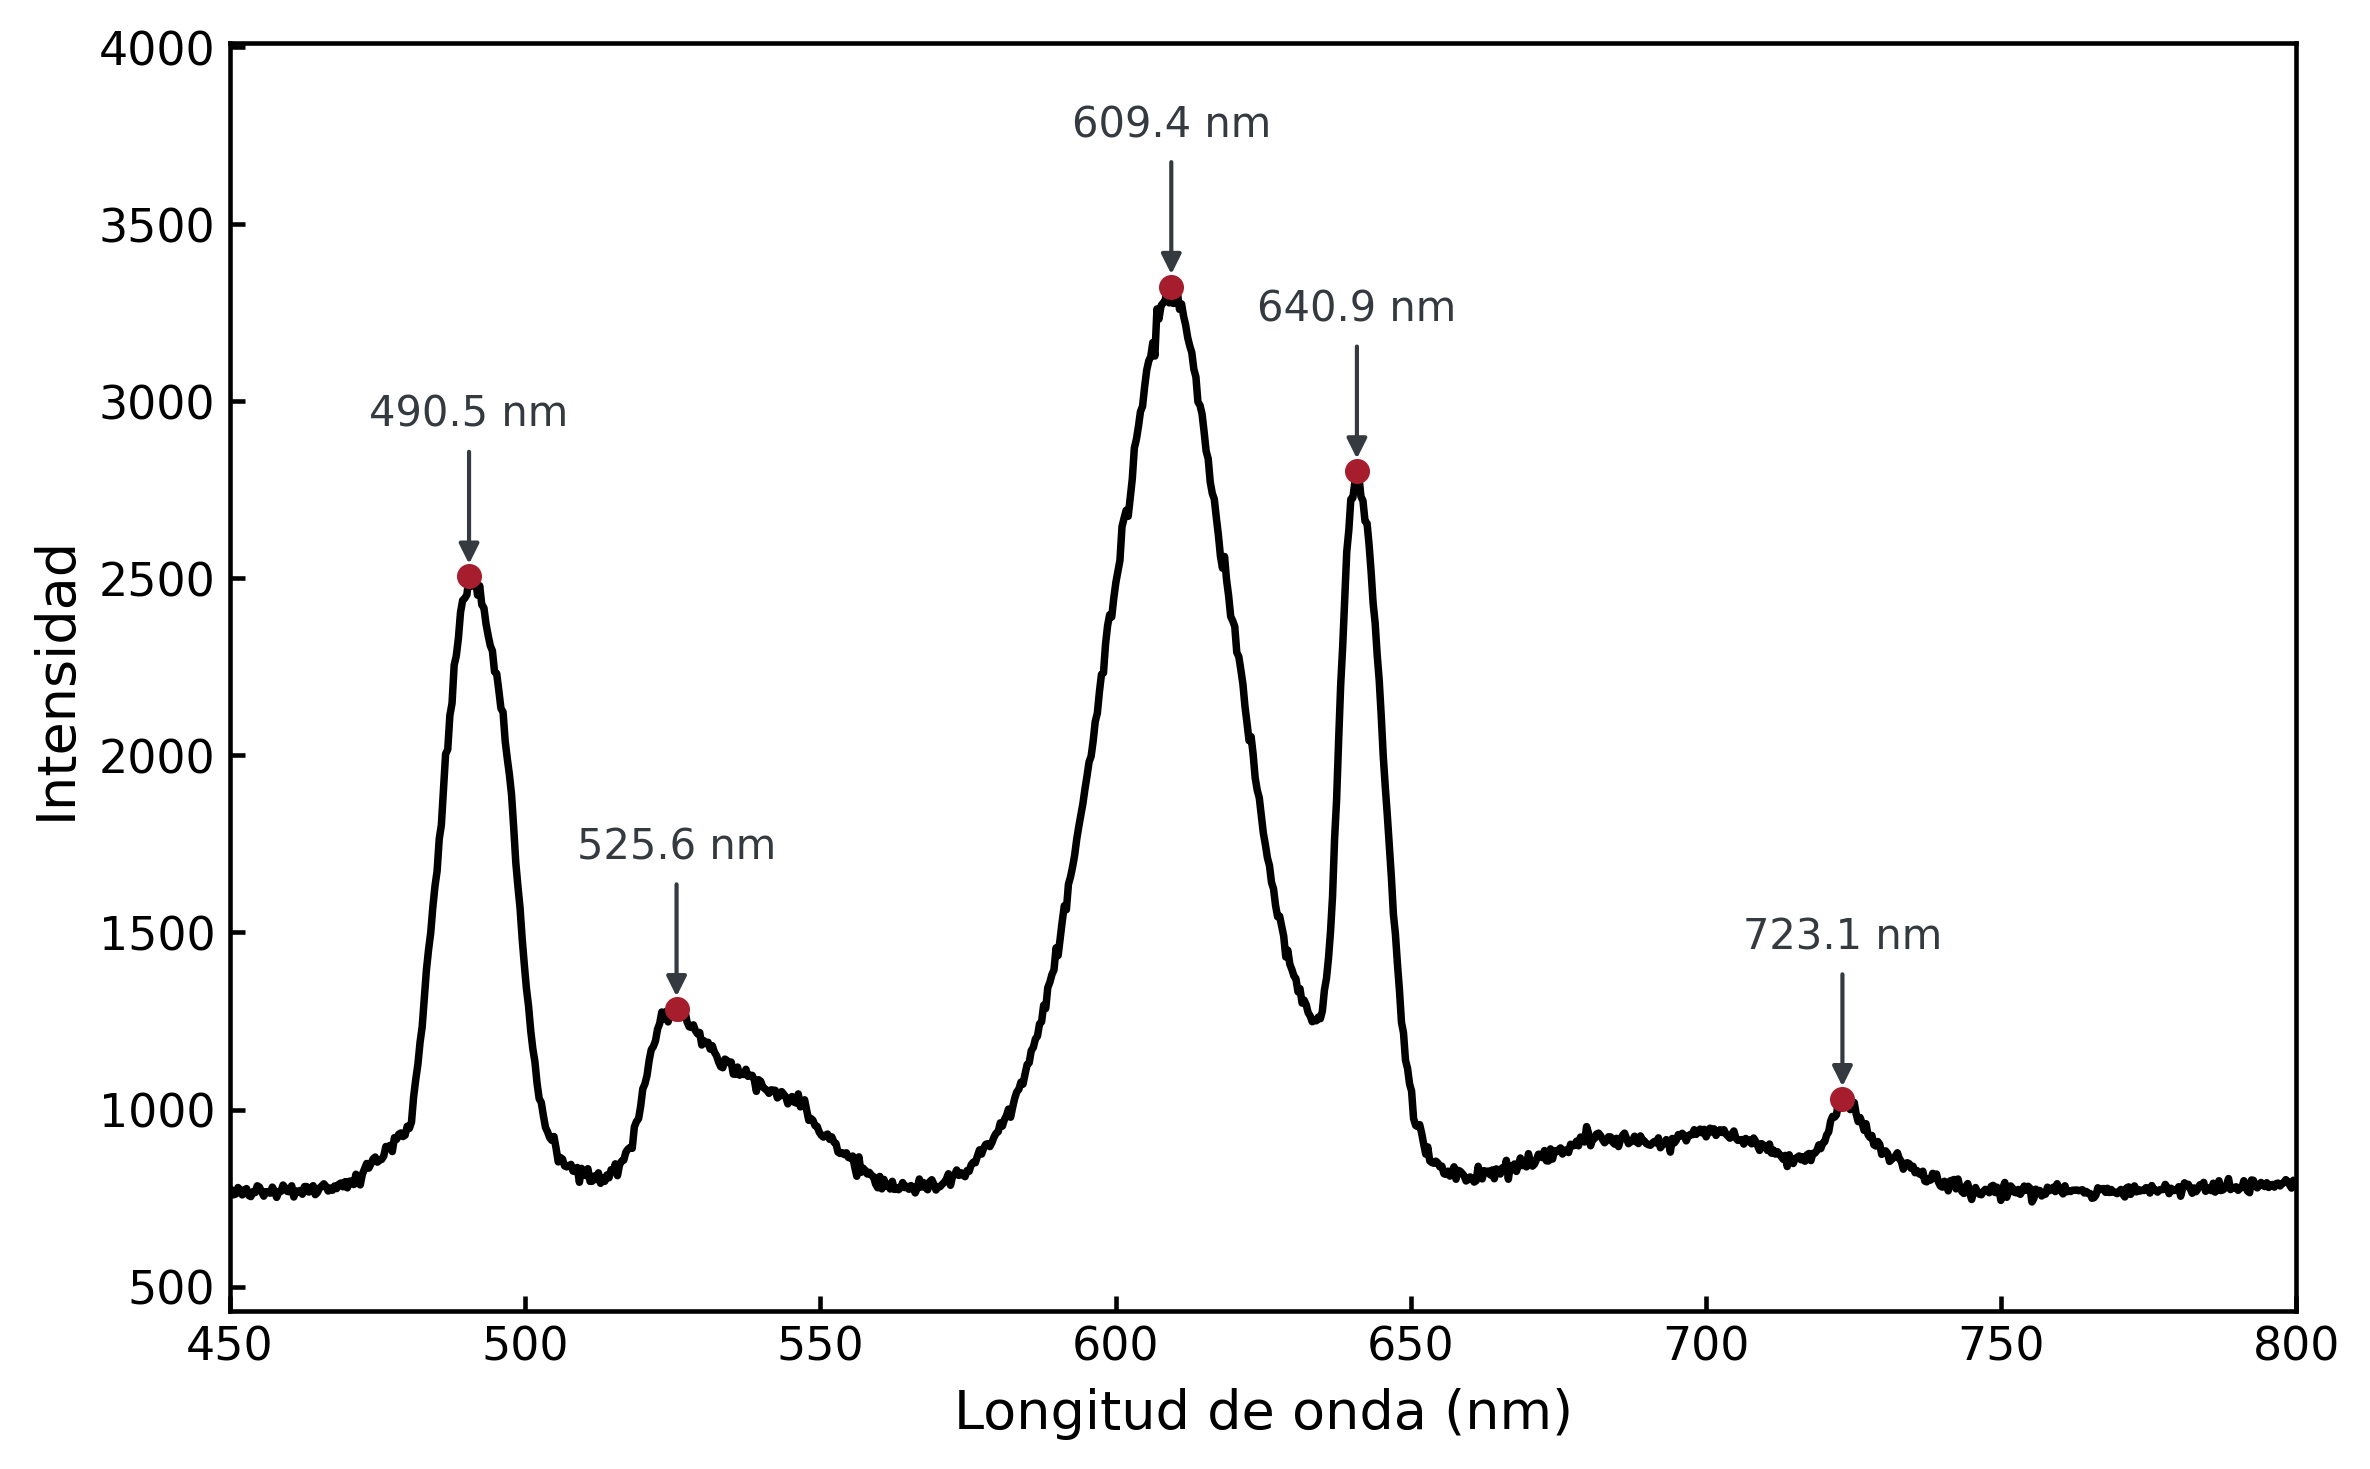
\includegraphics[scale=0.1]{figs/Pr-espec.png}
    \caption{Espectro de emisión de un cristal de Zn(PO$_3$)$_2$:Zn$_3$(PO$_4$)$_2$ ($49\%$, $49\%$, composición molar) dopado con Pr$_2$O$_3$ ($2\%$). Se señalan las intensidades máximas.}
    \label{fig:Pr_espectro}
\end{figure}

Se utilizó la Ecuación \ref{eq:numero_onda} y se
calcularon las siguientes energías: $E_{Pr_1} = 16408.51
\pm 1292.19\ \mathrm{cm}^{-1}$, $E_{Pr_2} = 15603.55
\pm 418.36\ \mathrm{cm}^{-1}$, $E_{Pr_3} = 20387.78
\pm 1500.07\ \mathrm{cm}^{-1}$, $E_{Pr_4} = 19024.43
\pm 2196.95\ \mathrm{cm}^{-1}$ y $E_{Pr_5} = 13828.96
\pm 48.25\ \mathrm{cm}^{-1}$. Finalmente,
para la elaboración del diagrama de energía de este ión
(Figura \ref{fig:Pr_diagrama-ener}) se consideraron el
rango de las incertidumbres de la energía, y se eligió el
que mejor correspondía con la información disponible
actualmente. \cite{Eu_Pr-literatura}

\begin{figure}%[H]
    \centering
    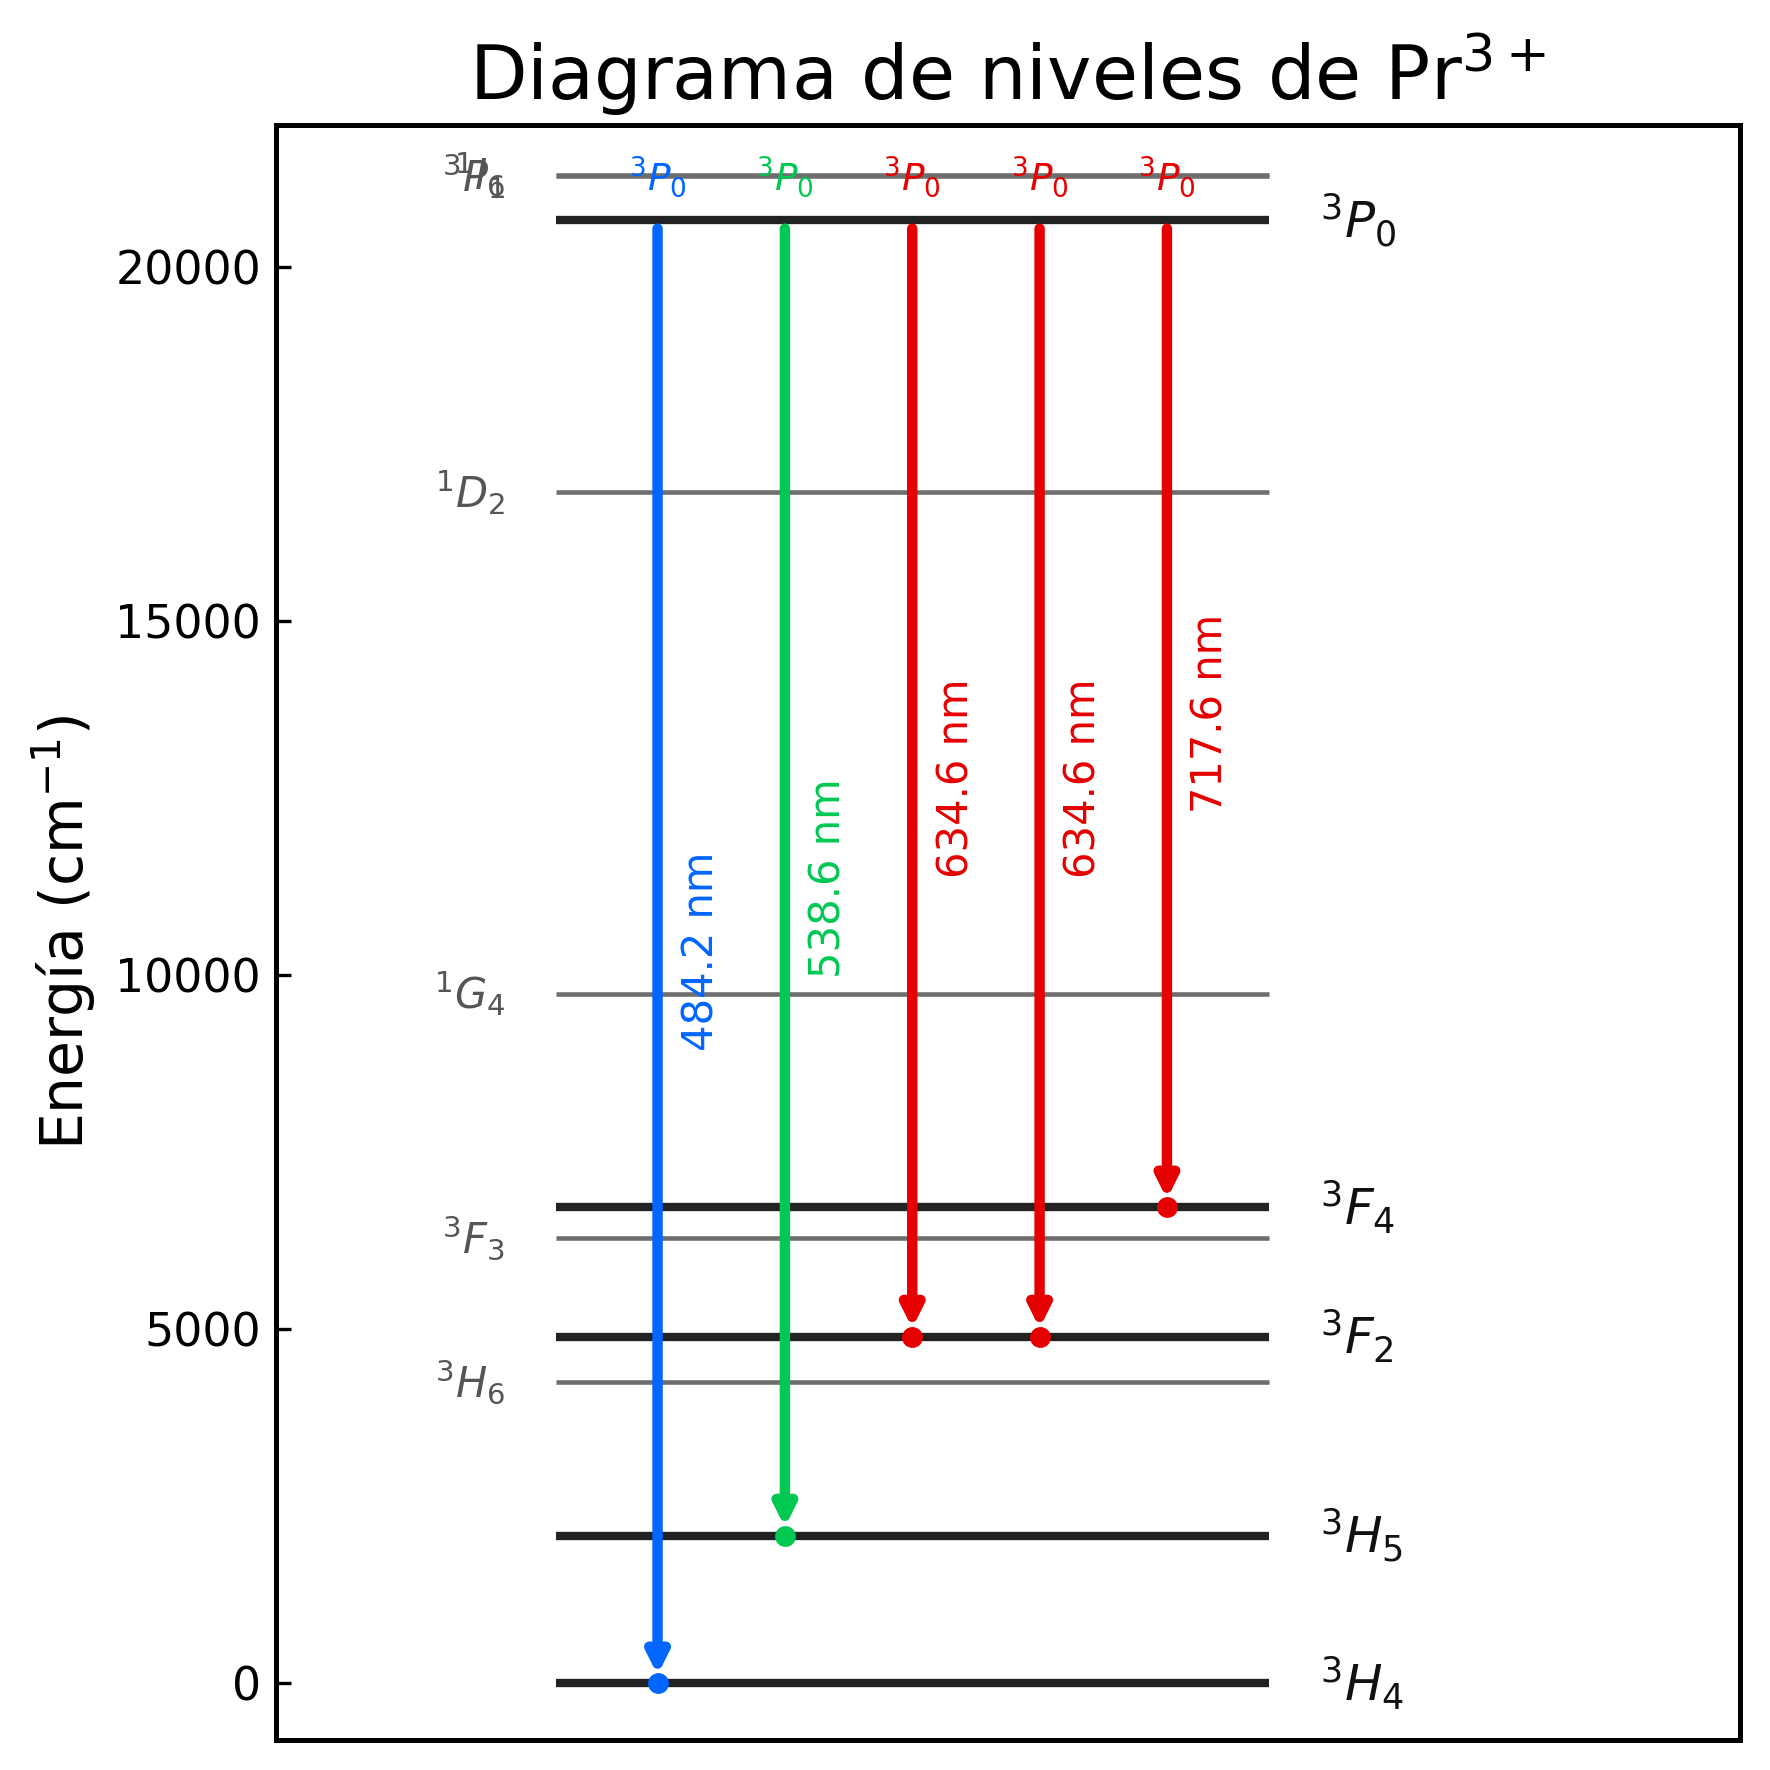
\includegraphics[scale=0.11]{figs/Pr-diag_ener.png}
    \caption{Diagrama de los niveles de energía de transición (fotoluminiscencia) del $Pr^{3+}$ calculado a partir de las intesidades máximas del espectro de emisión de un cristal de Zn(PO$_3$)$_2$:Zn$_3$(PO$_4$)$_2$ ($49\%$, $49\%$, composición molar) dopado con Pr$_2$O$_3$ ($2\%$). Se señalan las longitudes de onda correspondientes.}
    \label{fig:Pr_diagrama-ener}
\end{figure}\\
\textcolor{black}{\section{Conclusiones}}

\noindent Para el Dy$^{3+}$, se compararon los espectros obtenidos en dos matrices
vítreas distintas. En ambos se observaron bandas de emisión
características, aunque sus posiciones e intensidades relativas
presentaron variaciones. Esto sugiere que la matriz anfitriona influye
en el perfil de emisión del disprosio.

Para el Sm$^{3+}$, se compararon las mediciones del mismo vidrio de
fosfato de zinc realizadas con dos aparatos diferentes. Los máximos de
emisión aparecieron en longitudes de onda cercanas entre ambas
mediciones, por lo que las principales bandas se conservaron al cambiar
el instrumento. Las diferencias observadas pueden relacionarse con la
resolución, calibración y respuesta de cada aparato; por ello, las
intensidades absolutas no se compararon directamente.

En ambos casos, las bandas observadas se asociaron con transiciones
electrónicas características de los iones de tierras raras. Las
incertidumbres de longitud de onda se estimaron a partir de la anchura a
media altura de las bandas y las de número de onda se obtuvieron por
propagación. Estas incertidumbres son estimaciones espectrales y no
representan la incertidumbre instrumental.

Para el Tb$^{3+}$ se encontró que todos nuestros cálculos, considerando el rango de incertidumbre, de los niveles de transición que caracterizan su fotoluminiscencia están dentro de lo reportado en la literatura \cite{Tb-literatura}. A pesar de no tener un equipo altamente especializado, la configuración manual entre el láser y la fibra çoptica nos dio excelentes resultados.

Para el Eu$^{3+}$ se encontró casi la misma situación, solo hay una discrepancia con el decaimiento del $^5D_1$ al $^7F_6$, pues en la literatura \cite{Eu_Pr-literatura} se reporta que, para esa longitud de onda (aproximadamente), es del nivel $^5D_0$ al $^7F_4$.

Para el Pr$^{3+}$ también solo hay una discrepancia con un decaimiento en específico. Por la proximidad de estas dos intensidades y por el rango de incertidumbres, se encontró un mismo nivel de transcición: del $^3P_0$ al $^3F_2$. Se encontró \cite{Eu_Pr-literatura} que uno de ellos debería de caer al nivel $^3H_6$, aunque claro, con una longitud de onda un poco distinta.\\
\ifCLASSOPTIONcaptionsoff
  \newpage
\fi
\begin{thebibliography}{3}

	\bibitem{PELS55}
	Hamilton Instrument. (s.f.). “Perkin Elmer LS55 Luminescence Spectrometer”. Hamilton Instrument. \url{https://www.hamiltoninstrument.com/index.php?route=product/product\&product_id=199}

    \bibitem{Tb-literatura}
	J. Zmojda, M. Kochanowicz, P. Miluski, D. Dorosz. (2014). “Side-Detecting Optical Fiber Doped with Tb$^{3+}$ for Ultraviolet Sensor Application”. Fibers, 2(2), 150--157. DOI: 10.3390/fib2020150.

\bibitem{Eu_Pr-literatura}
B. Klimesz, G. Dominiak-Dzik, P. Solarz, M. Żelechower y W. Ryba-Romanowski,
``Optical study of GeO$_2$--PbO--PbF$_2$ oxyfluoride glass singly doped with Pr$^{3+}$, Nd$^{3+}$, Sm$^{3+}$ and Eu$^{3+}$'', \textit{Journal of Alloys and Compounds}, \textbf{403}, 76--85 (2005). https://doi.org/10.1016/j.jallcom.2005.05.033
\bibitem{RighiniFerrari2005}
Righini, G. C., y Ferrari, M. (2005).
“Photoluminescence of rare-earth-doped glasses”.
\textit{Rivista del Nuovo Cimento}, 28(12).
\url{https://doi.org/10.1393/ncr/i2006-10010-8}

\bibitem{Cheng2018}
Cheng, P., Zhou, Y., Su, X., Zhou, M., Zhou, Z., y Shao, H. (2018).
“Pr$^{3+}$/Er$^{3+}$ co-doped tellurite glass with ultra-broadband
near-infrared fluorescence emission”.
\textit{Journal of Luminescence}, 197, 31--37.
\url{https://doi.org/10.1016/j.jlumin.2018.01.005}
\end{thebibliography}
\textcolor{black}{\section{Anexo}}

% Cambia de dos columnas a una página completa.
% También provoca el salto a la siguiente página.
\onecolumn

\thispagestyle{plain}

% =====================================================
% FILA 1
% =====================================================

\noindent
\begin{minipage}[t][0.29\textheight][t]{0.48\textwidth}
    \centering

    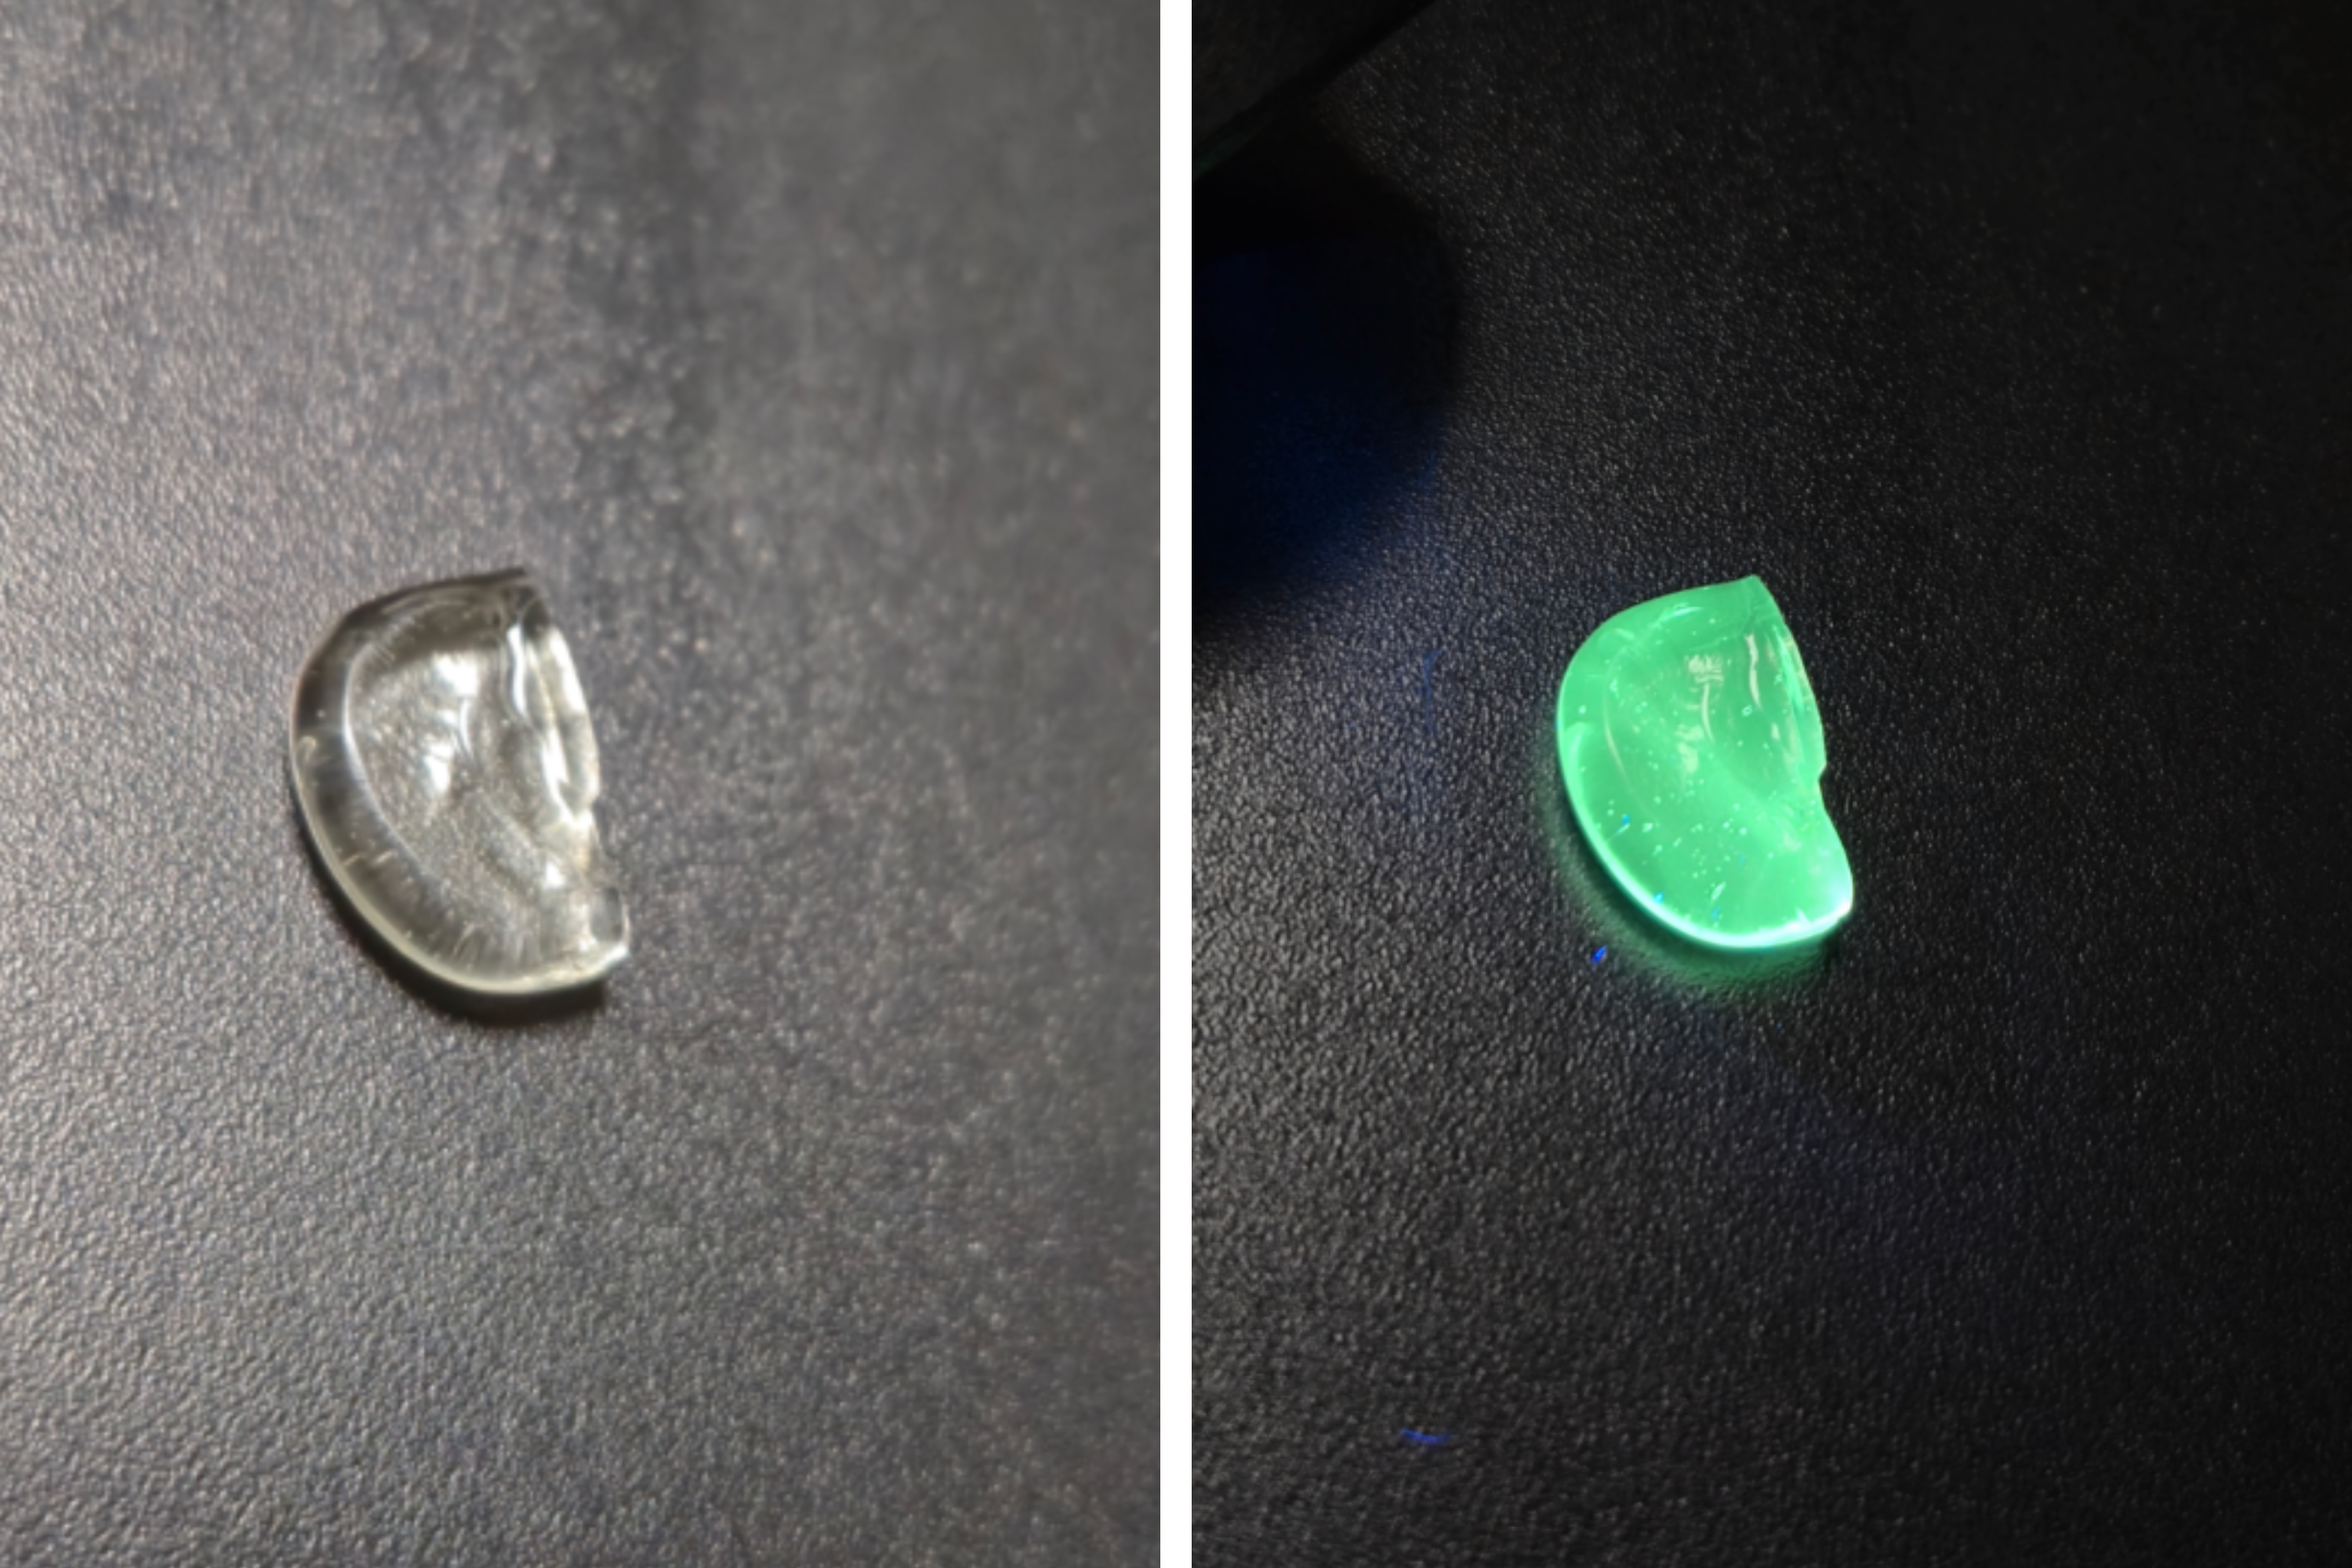
\includegraphics[
        width=\linewidth,
        height=0.22\textheight,
        keepaspectratio
    ]{figs/Dy_Mg-fotos.png}

    \captionof{figure}{
        Muestra de Mg(PO$_3$)$_2$:Mg$_3$(PO$_4$)$_2$:Dy$_2$O$_3$
        (composición molar: $49.25\%$, $49.25\%$, $1\%$).
        A la derecha presenta el fenómeno de fotoluminiscencia;
        excitado con una luz de $365$ nm.
    }
    \label{fig:Dy_Mg-fotos}
\end{minipage}%
\hfill
\begin{minipage}[t][0.29\textheight][t]{0.48\textwidth}
    \centering

    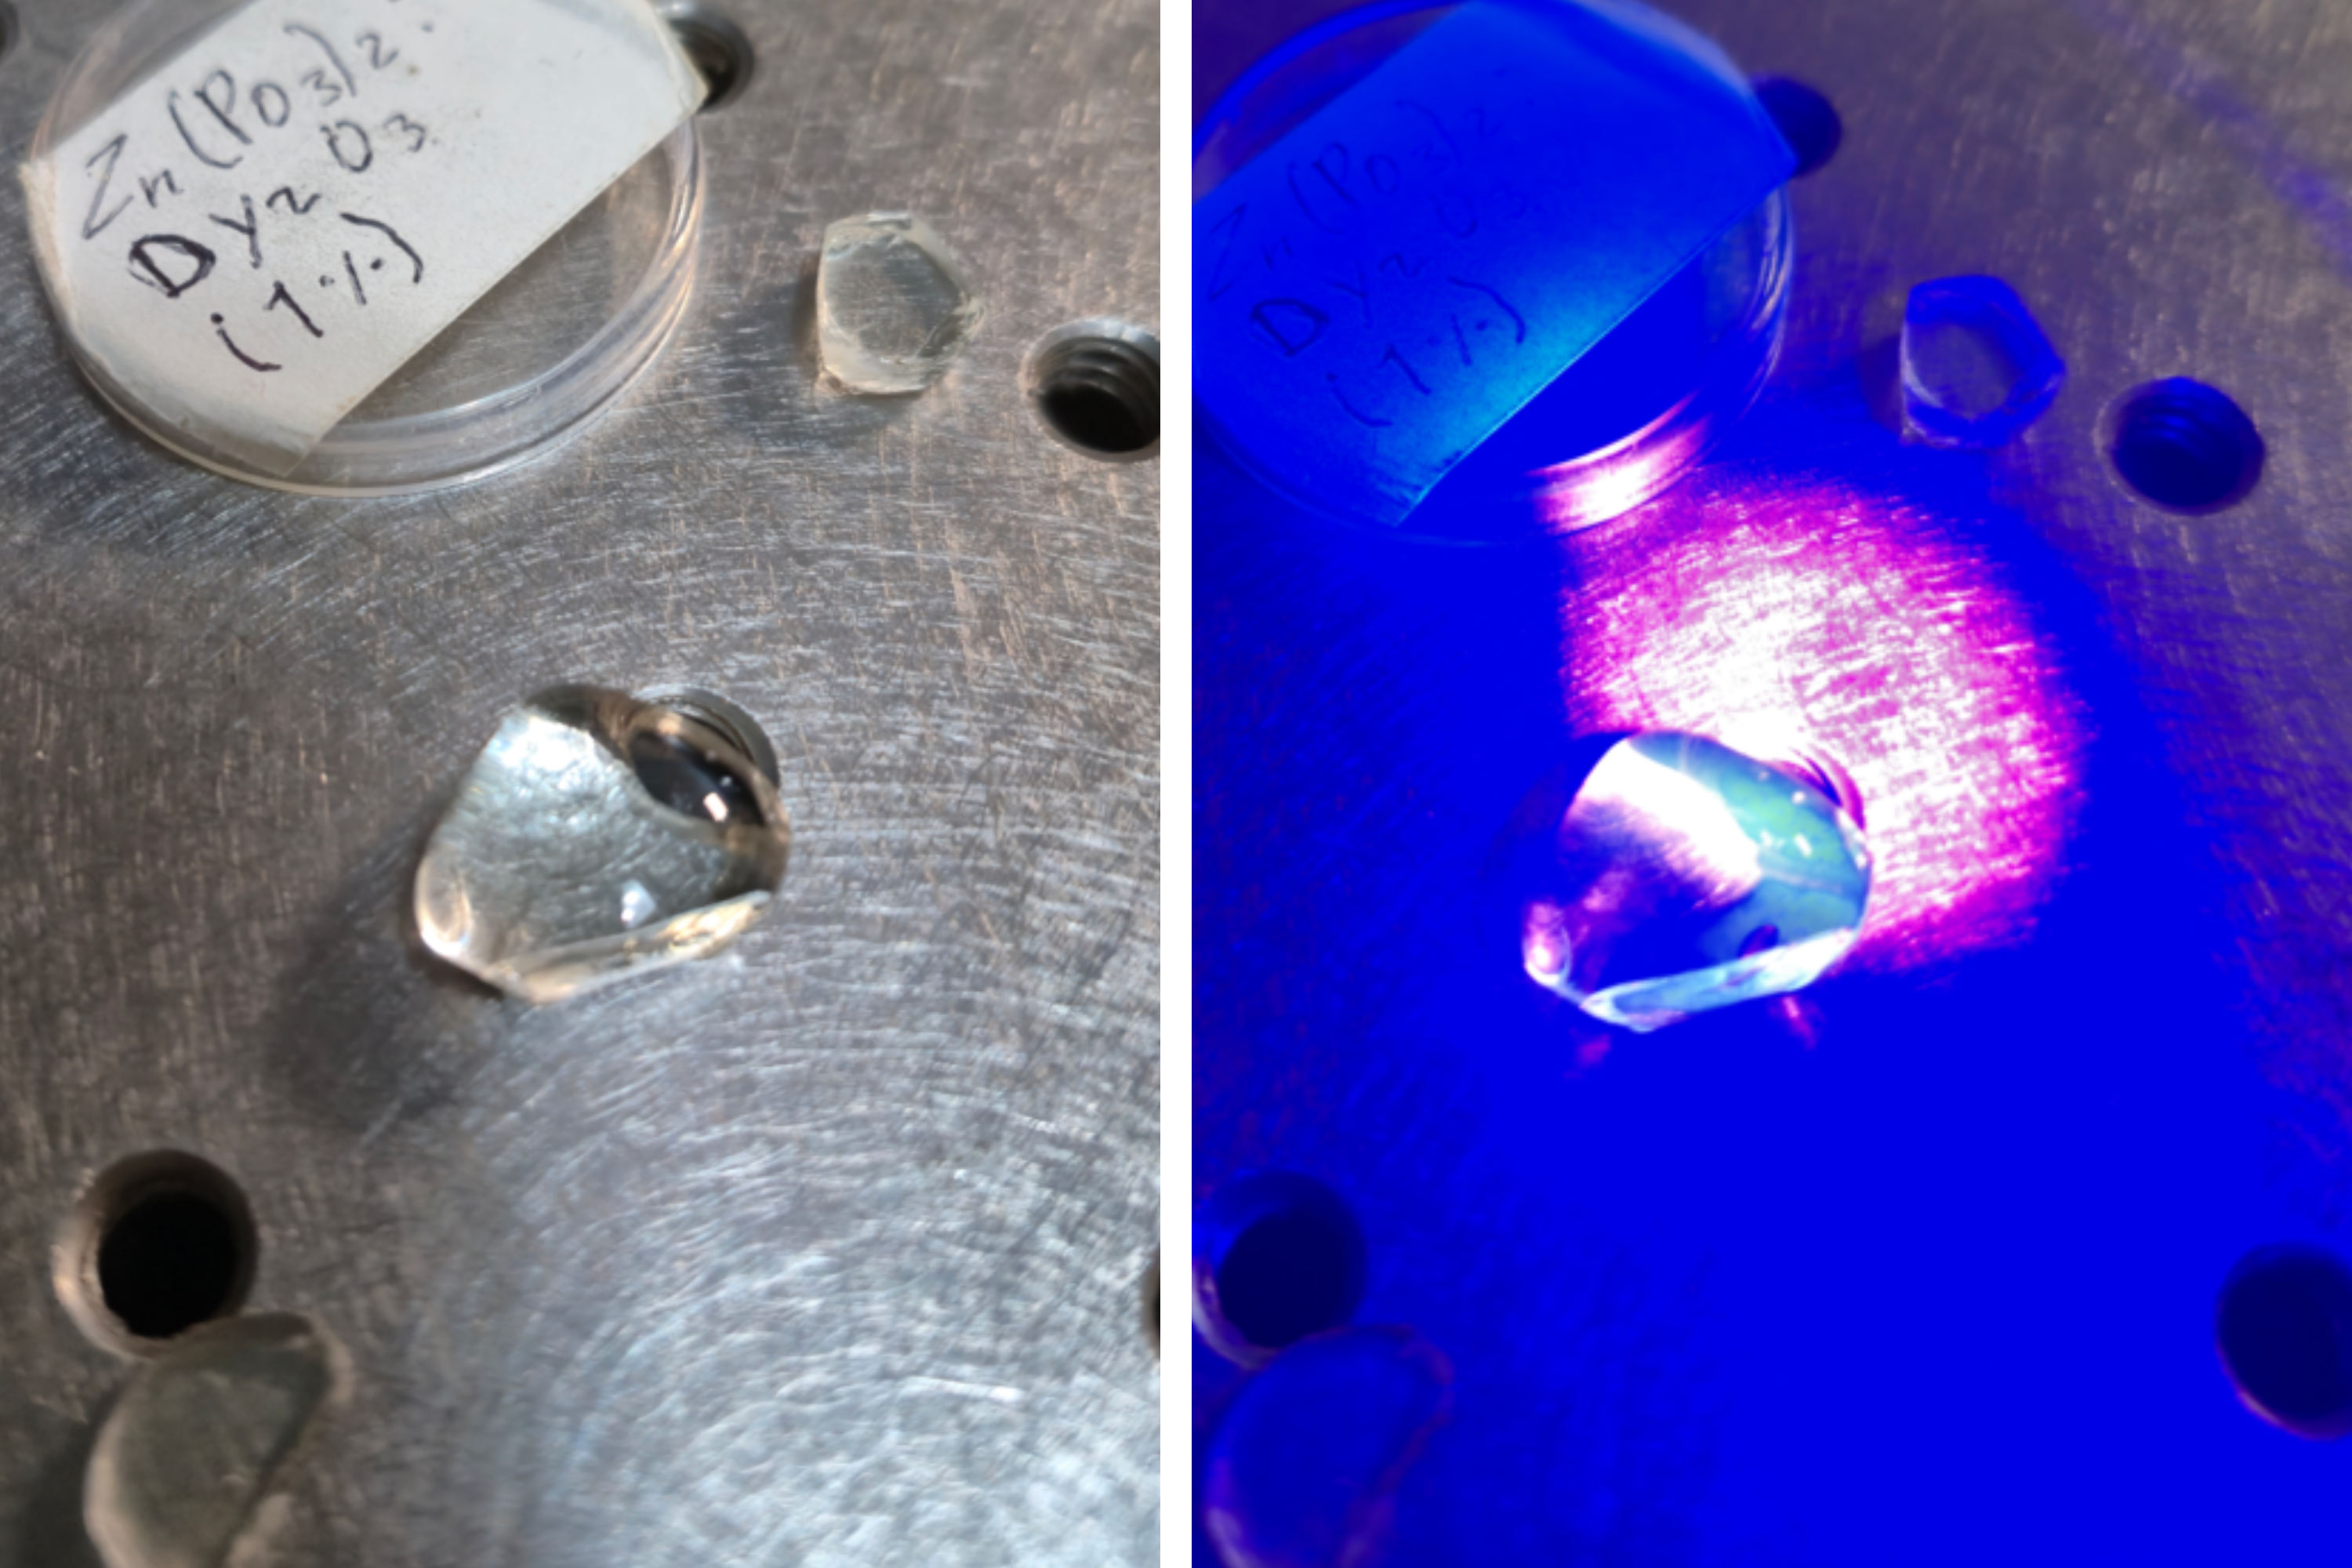
\includegraphics[
        width=\linewidth,
        height=0.22\textheight,
        keepaspectratio
    ]{figs/Dy_Zn-fotos.png}

    \captionof{figure}{
        Muestra de Zn(PO$_3$)$_2$:Dy$_2$O$_3$
        (composición molar: $99\%$, $1\%$).
        A la derecha presenta el fenómeno de fotoluminiscencia;
        excitado con una luz de $365$ nm.
    }
    \label{fig:Dy_Zn-fotos}
\end{minipage}

\vfill

% =====================================================
% FILA 2
% =====================================================

\noindent
\begin{minipage}[t][0.29\textheight][t]{0.48\textwidth}
    \centering

    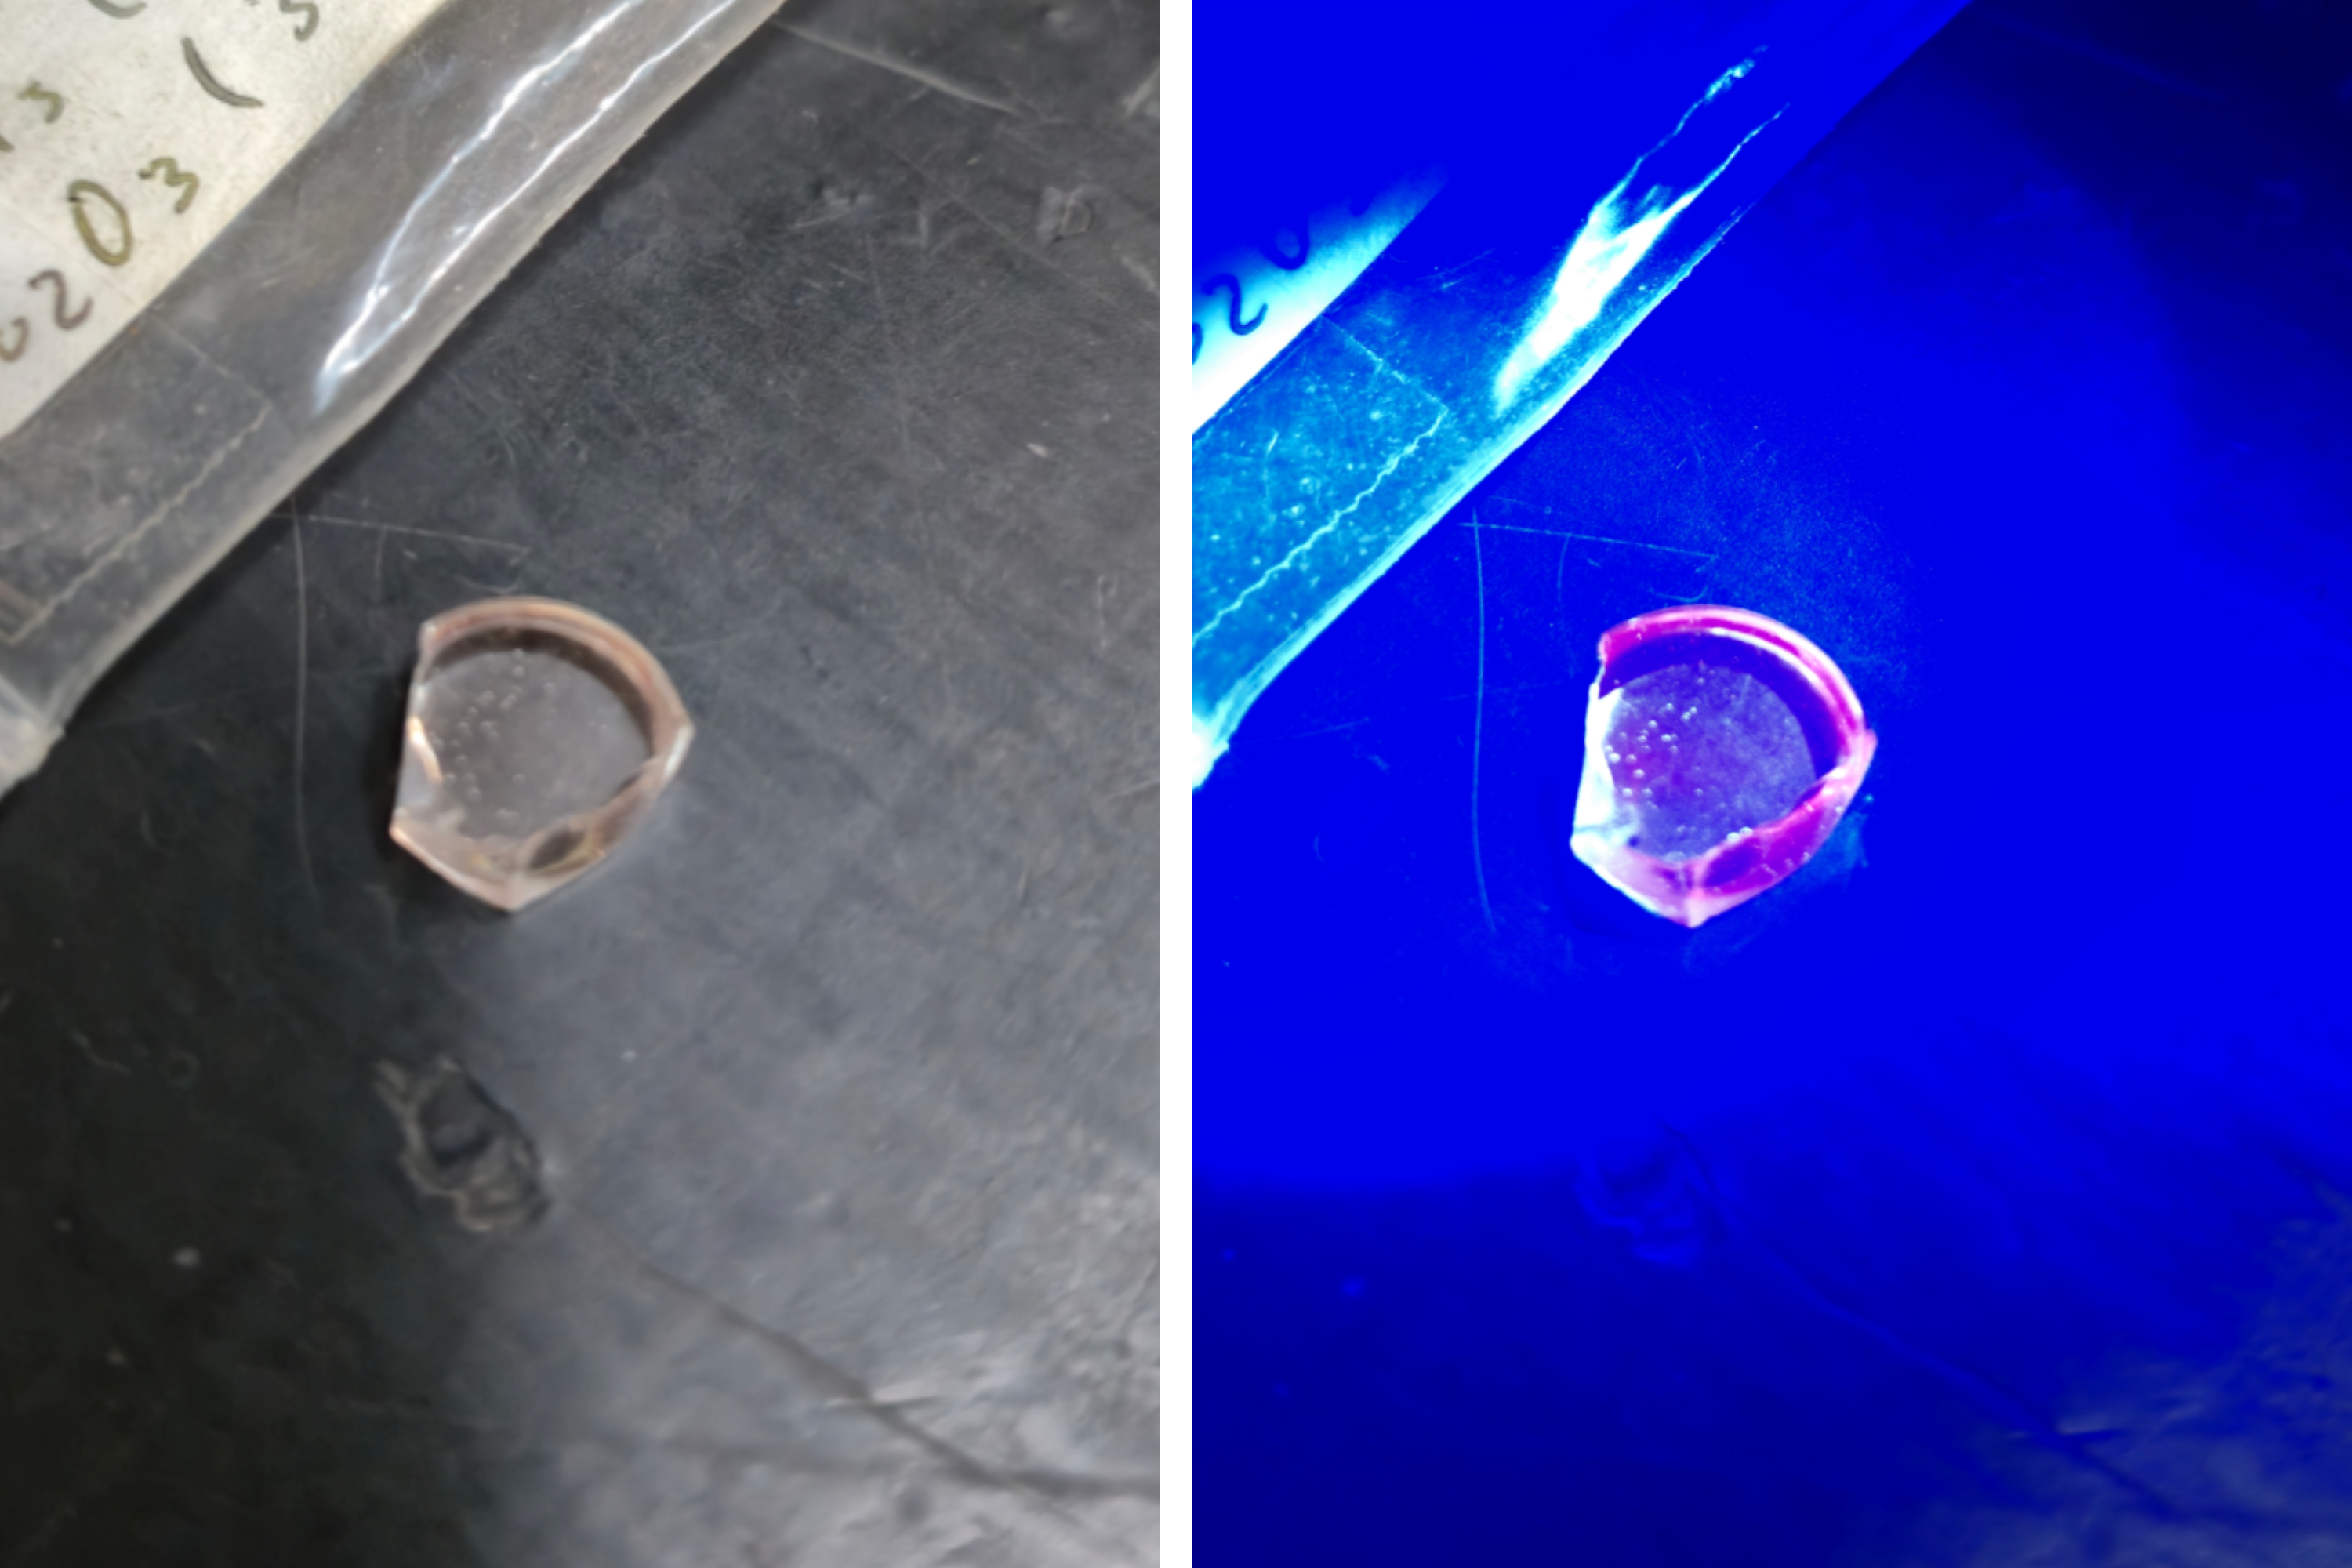
\includegraphics[
        width=\linewidth,
        height=0.22\textheight,
        keepaspectratio
    ]{figs/Eu-fotos.png}

    \captionof{figure}{
        Muestra de Mg(PO$_3$)$_2$:Mg$_3$(PO$_4$)$_2$:SnCl$_3$:Eu$_2$O$_3$
        (composición molar: $49\%$, $48\%$, $1\%$, $3\%$).
        A la derecha presenta el fenómeno de fotoluminiscencia;
        excitado con una luz de $458$ nm.
    }
    \label{fig:Eu-fotos}
\end{minipage}%
\hfill
\begin{minipage}[t][0.29\textheight][t]{0.48\textwidth}
    \centering

    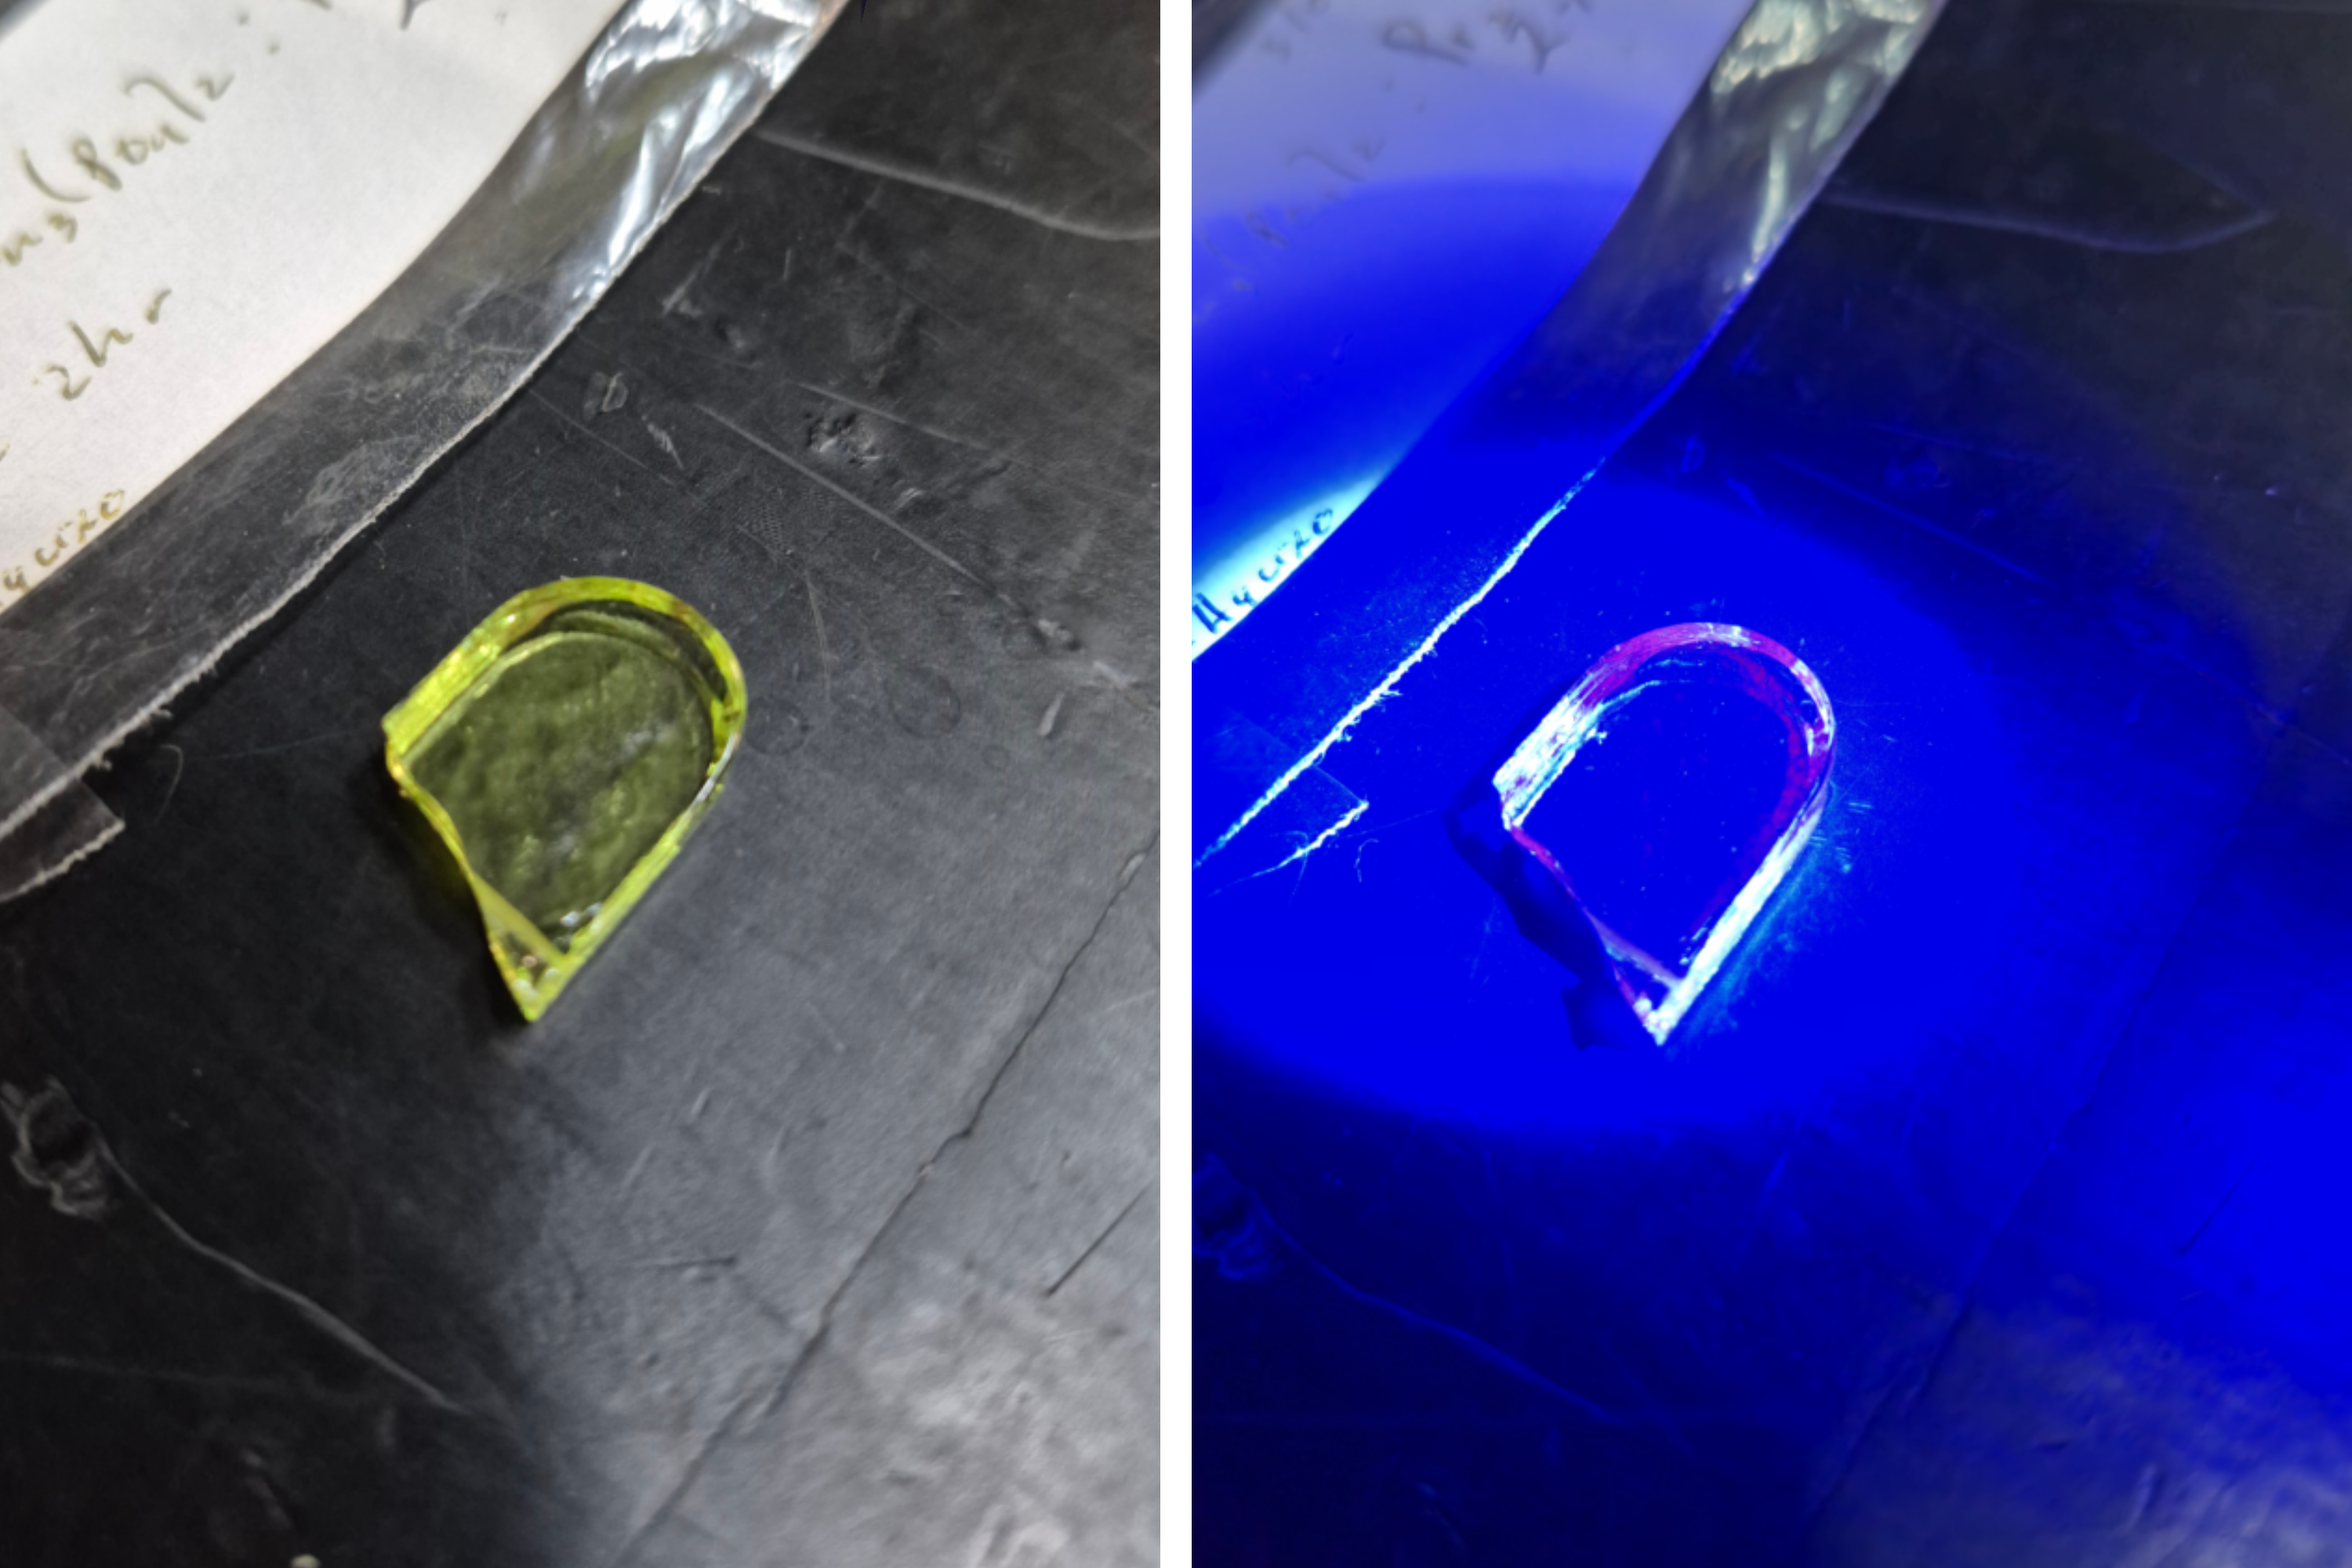
\includegraphics[
        width=\linewidth,
        height=0.22\textheight,
        keepaspectratio
    ]{figs/Pr-fotos.png}

    \captionof{figure}{
        Muestra de Zn(PO$_3$)$_2$:Zn$_3$(PO$_4$)$_2$:Pr$_2$O$_3$
        (composición molar: $49\%$, $49\%$, $2\%$).
        A la derecha presenta el fenómeno de fotoluminiscencia;
        excitado con una luz de $458$ nm.
    }
    \label{fig:Pr-fotos}
\end{minipage}

\vfill

% =====================================================
% FILA 3
% =====================================================

\noindent
\begin{minipage}[t][0.29\textheight][t]{0.48\textwidth}
    \centering

    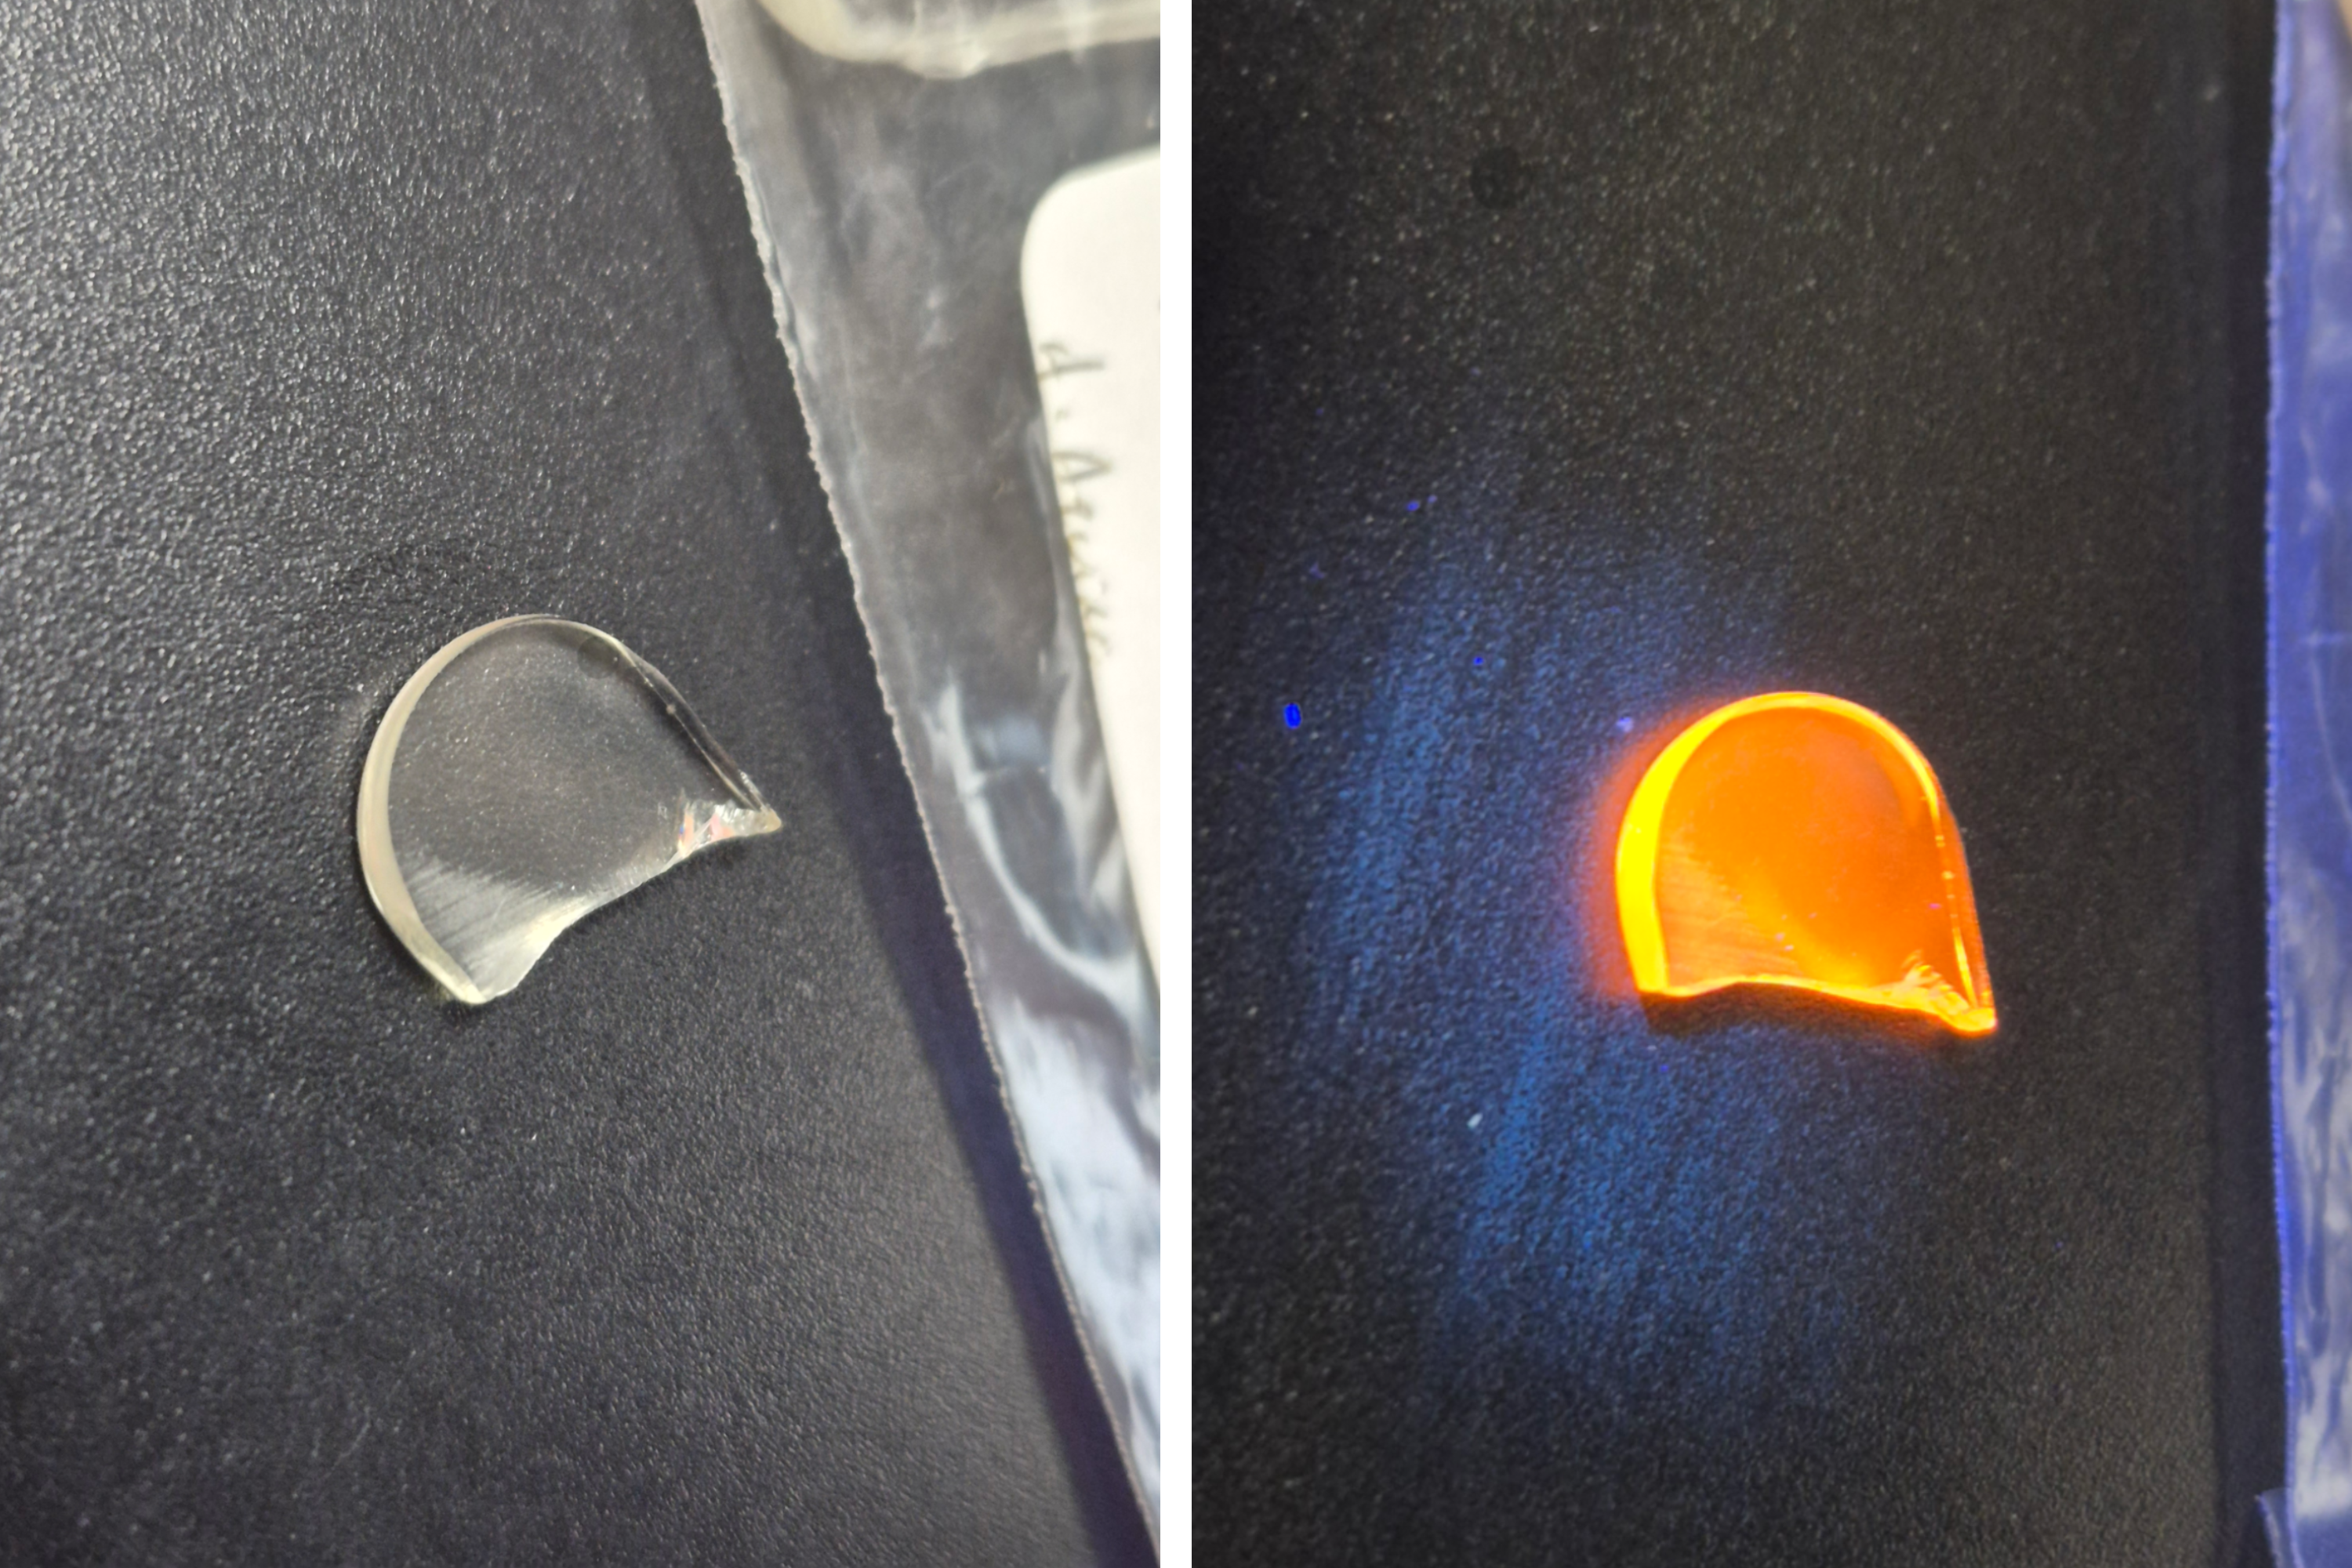
\includegraphics[
        width=\linewidth,
        height=0.22\textheight,
        keepaspectratio
    ]{figs/Sm-fotos.png}

    \captionof{figure}{
        Muestra de Zn(PO$_3$)$_2$:Zn$_3$(PO$_4$)$_2$:Sm$_2$O$_3$
        (composición molar: $49.5\%$, $49.5\%$, $1\%$).
        A la derecha presenta el fenómeno de fotoluminiscencia;
        excitado con una luz de $365$ nm.
    }
    \label{fig:Sm-fotos}
\end{minipage}%
\hfill
\begin{minipage}[t][0.29\textheight][t]{0.48\textwidth}
    \centering

    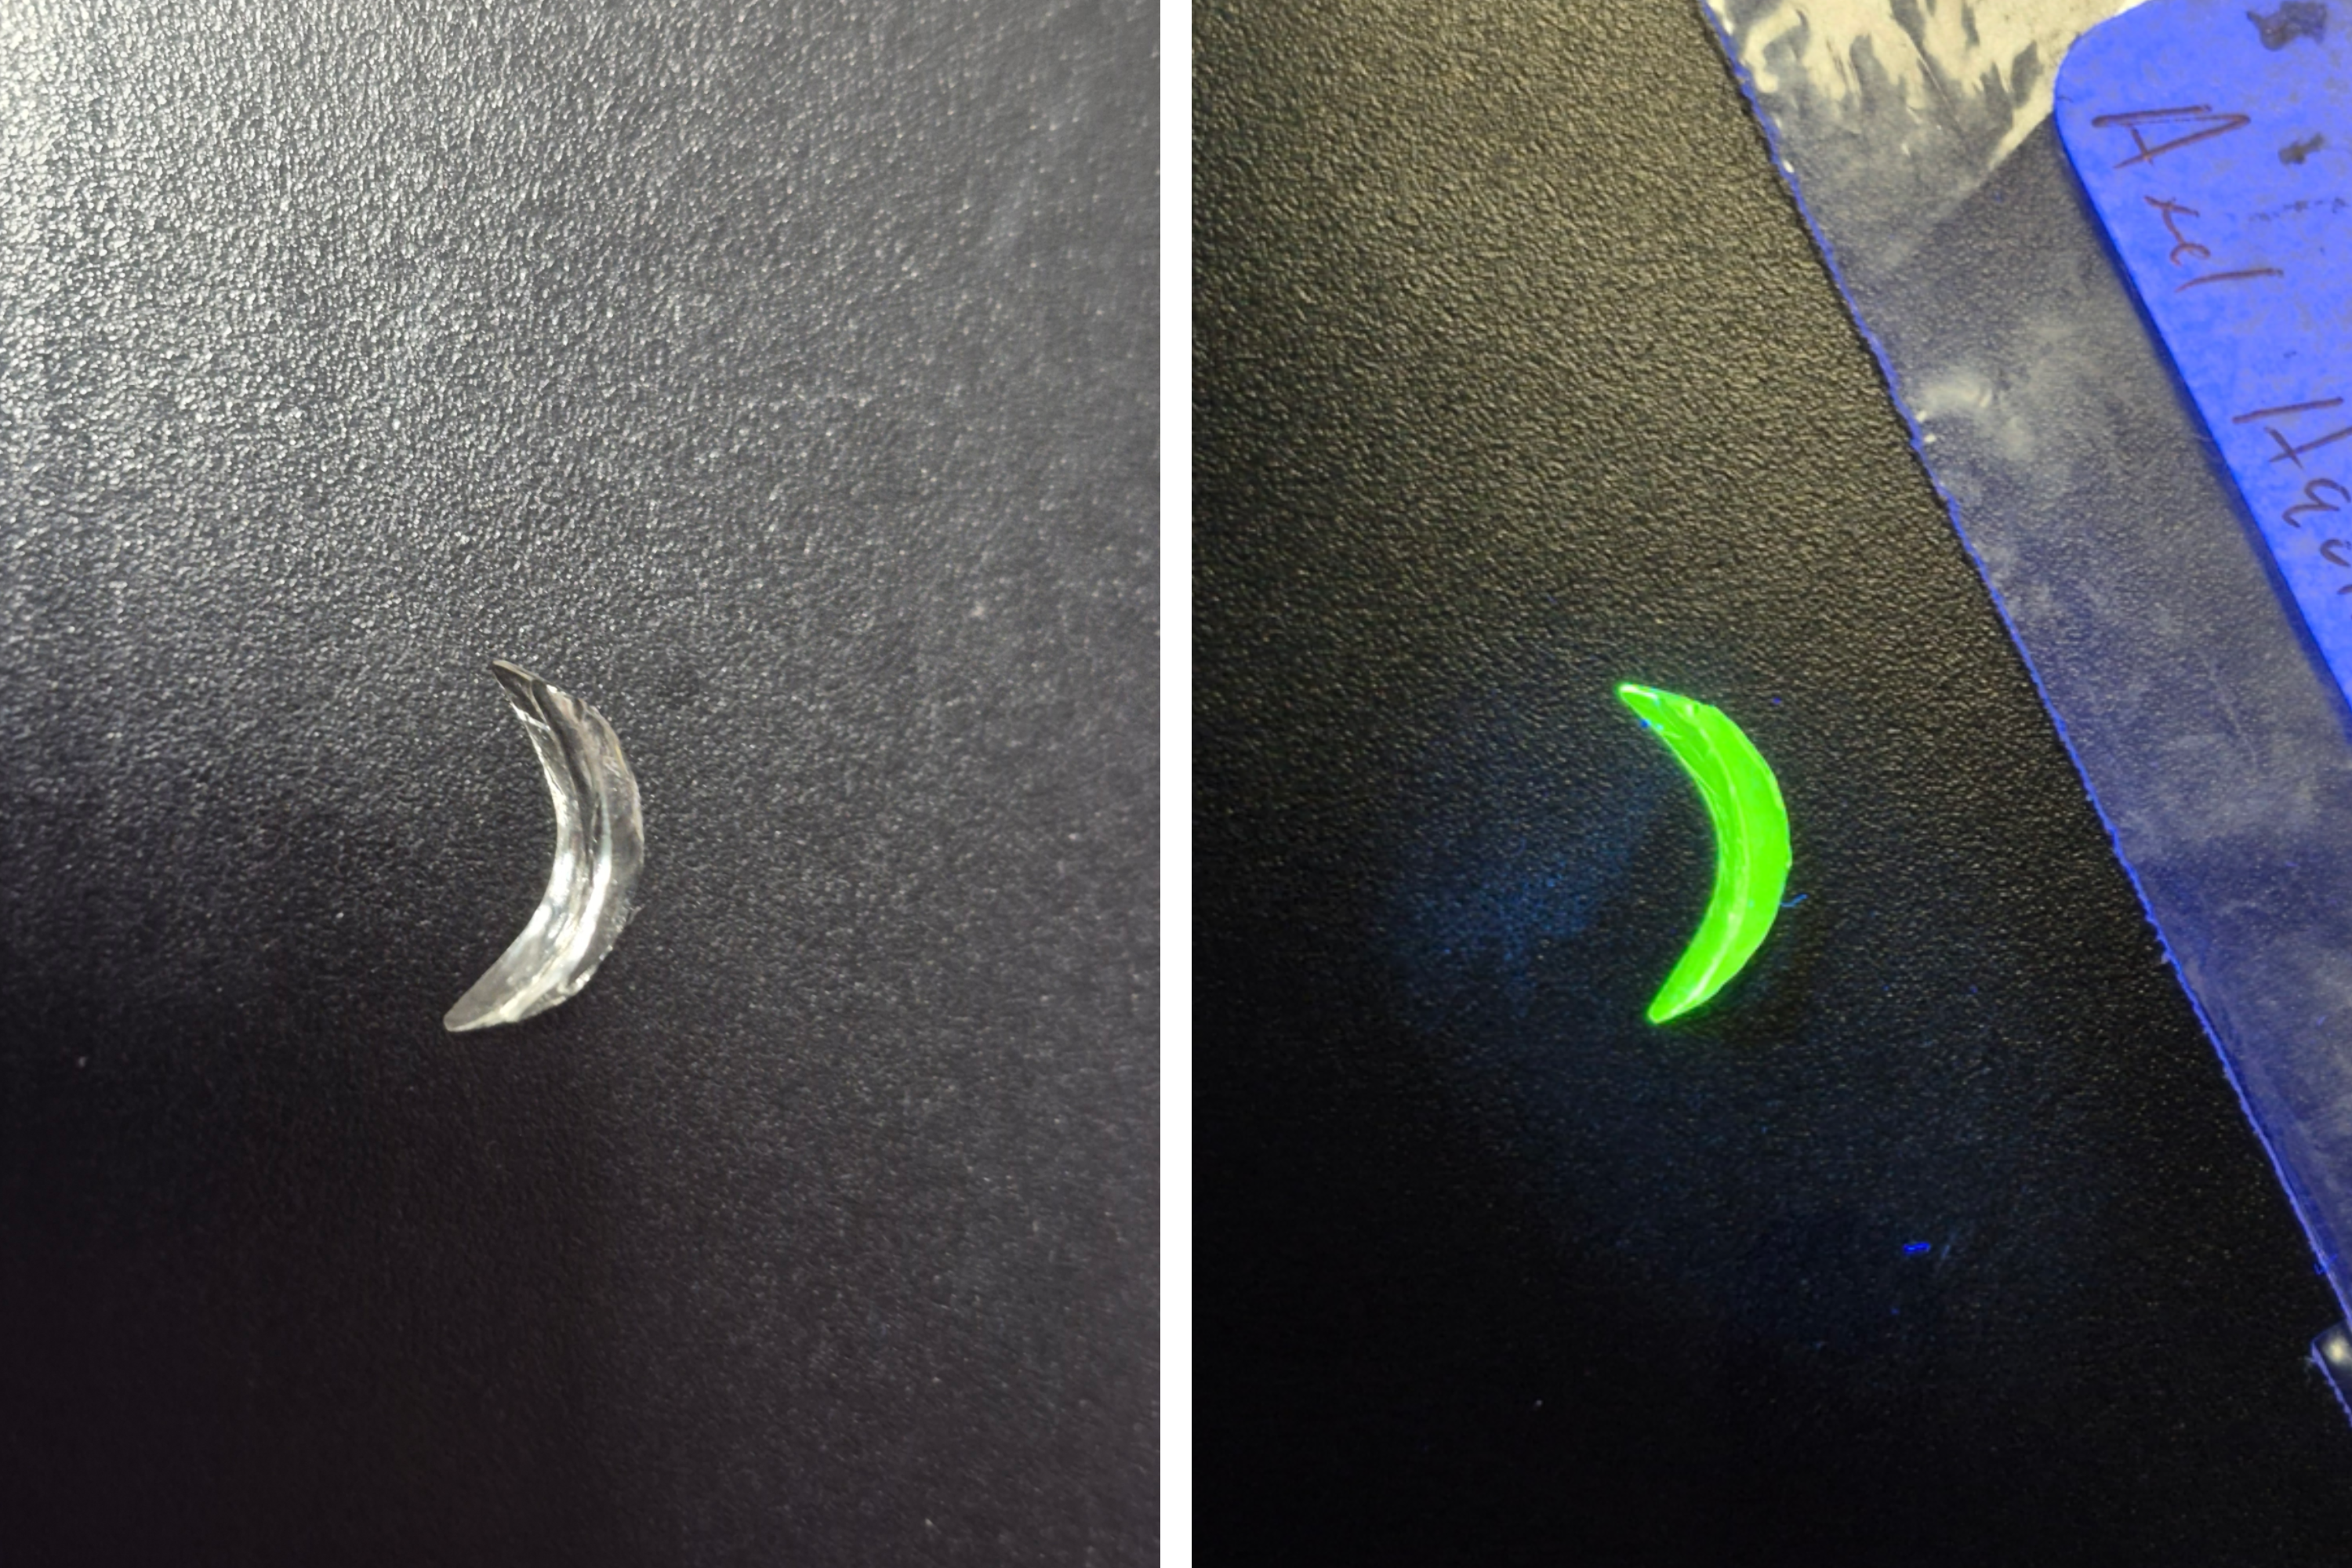
\includegraphics[
        width=\linewidth,
        height=0.22\textheight,
        keepaspectratio
    ]{figs/Tb-fotos.png}

    \captionof{figure}{
        Muestra de Li$_2$B$_4$O$_7$:Tb$_4$O$_7$
        (composición molar: $98\%$, $2\%$).
        A la derecha presenta el fenómeno de fotoluminiscencia;
        excitado con una luz de $366$ nm.
    }
    \label{fig:Tb-fotos}
\end{minipage}

\end{document}